% !TEX program = xelatex
\documentclass[12pt,a4paper]{scrartcl}

\usepackage{fontspec}
\usepackage{polyglossia}
\setdefaultlanguage{portuguese}
\PolyglossiaSetup{portuguese}{indentfirst=false}
\setmainfont{Latin Modern Roman}[Scale=1.08]
\setsansfont{Latin Modern Sans}[Scale=1.08]
\setmonofont{Latin Modern Mono}[Scale=1.00]
\usepackage{unicode-math}
\setmathfont{Latin Modern Math}[Scale=1.08]

\usepackage{amsmath}
\usepackage{mathtools}

\usepackage[a4paper,top=2.8cm,bottom=2.8cm,left=2.6cm,right=2.6cm,
            headheight=16pt]{geometry}
\usepackage{microtype}
\usepackage{xcolor}
\usepackage{booktabs}
\usepackage{array}
\usepackage{tabularx}
\usepackage{enumitem}
\usepackage{titlesec}
\usepackage{fancyhdr}
\usepackage{graphicx}
\usepackage{subcaption}
\usepackage{caption}
\usepackage{float}
\graphicspath{{img/}}
\usepackage{csquotes}
\usepackage{needspace}
\usepackage{tcolorbox}
\tcbuselibrary{skins,breakable}
\definecolor{accent}{HTML}{5B8E3F}
\definecolor{accentdark}{HTML}{406A2A}
\definecolor{earth}{HTML}{825432}
\definecolor{ink}{HTML}{1F1F23}
\definecolor{muted}{HTML}{4E4E58}
\definecolor{bg}{HTML}{FBF6E9}
\definecolor{rule}{HTML}{D8D1BC}
\definecolor{linkc}{HTML}{2D5A1F}

\usepackage[colorlinks=true,
            linkcolor=linkc,
            urlcolor=linkc,
            citecolor=linkc,
            bookmarks=true,bookmarksopen=true,
            pdftitle={Block Round — A Matemática do Projeto},
            pdfauthor={Vinícius Rodrigues de Souza}]{hyperref}

\color{ink}

\titleformat{\section}
  {\sffamily\Large\bfseries\color{accent}}{\thesection.}{0.6em}{}
\titleformat{\subsection}
  {\sffamily\large\bfseries\color{accent!85!ink}}{\thesubsection}{0.6em}{}
\titlespacing*{\section}{0pt}{1.2\baselineskip}{0.6\baselineskip}
\titlespacing*{\subsection}{0pt}{0.8\baselineskip}{0.3\baselineskip}

\pagestyle{fancy}
\fancyhf{}
\fancyhead[L]{\small\sffamily\bfseries\color{accent}BLOCK ROUND}
\fancyhead[R]{\small\sffamily\color{muted}A Matemática do Projeto}
\fancyfoot[L]{\small\sffamily\color{muted}Block Round — Documento técnico}
\fancyfoot[R]{\small\sffamily\color{muted}Página \thepage}
\renewcommand{\headrulewidth}{0.4pt}
\renewcommand{\footrulewidth}{0.4pt}
\renewcommand{\headrule}{{\color{rule}\hrule height \headrulewidth}}
\renewcommand{\footrule}{{\color{rule}\vskip-\footrulewidth\hrule height \footrulewidth\vskip-\footrulewidth}}

\newtcolorbox{formula}{
  colback=bg, colframe=rule, boxrule=0.4pt, arc=2pt,
  left=10pt,right=10pt,top=8pt,bottom=8pt,
  before skip=8pt, after skip=8pt,
  fontupper=\color{accentdark}, breakable,
  before={\par\needspace{4\baselineskip}}
}

\newtcolorbox{minec}{
  colback=accent!7, colframe=accent!50!rule, boxrule=0.6pt, arc=2pt,
  left=10pt,right=10pt,top=8pt,bottom=8pt,
  before skip=10pt, after skip=10pt,
  breakable,
  before={\par\needspace{5\baselineskip}}
}

\setlength{\parskip}{0.75em}
\setlength{\parindent}{0pt}
\linespread{1.10}

\newcommand{\code}[1]{\texttt{\small #1}}
\newcommand{\acc}[1]{\textcolor{accent}{\textbf{#1}}}
\newcommand{\cmd}[1]{\textcolor{earth}{\texttt{\small #1}}}

\begin{document}

\begin{titlepage}
  \centering
  \vspace*{3.5cm}
  {\sffamily\bfseries\fontsize{56}{60}\selectfont \color{accent} Block Round\par}
  \vspace{0.7cm}
  {\sffamily\LARGE\color{muted} A Matemática do Projeto\par}
  \vspace{1.4cm}
  {\color{rule}\rule{0.6\textwidth}{0.6pt}\par}
  \vspace{0.9cm}
  \begin{minipage}{0.82\textwidth}
    \centering\color{ink}\large
    Documentação técnica e didática dos fundamentos matemáticos empregados no gerador de círculos, elipses, esferas e elipsóides \emph{renderizados com texturas de blocos de Minecraft}. Para cada conceito, apresentam-se a definição formal, a justificação geométrica, a correspondência direta com o código-fonte do projeto e a tradução prática para os comandos de construção no jogo (\cmd{/fill}, \cmd{/clone}, \cmd{//sphere}).
  \end{minipage}
  \vspace{0.9cm}\\
  {\color{rule}\rule{0.6\textwidth}{0.6pt}\par}
  \vspace{2cm}
  \begin{minipage}{0.78\textwidth}
    \centering\sffamily\small\color{muted}
    \textbf{Áreas abordadas:} geometria analítica $\cdot$ rasterização discreta $\cdot$ topologia digital $\cdot$ cálculo integral $\cdot$ álgebra linear $\cdot$ trigonometria $\cdot$ aritmética de inventário $\cdot$ mapeamento de texturas $\cdot$ simetria octaédrica.
  \end{minipage}
\end{titlepage}

\renewcommand{\contentsname}{\color{accent}Sumário}
\tableofcontents
\thispagestyle{fancy}
\newpage

% =============================================================================
\section{Visão geral: natureza matemática do problema}

O Block Round é um gerador de formas arredondadas \emph{texturizadas com blocos de Minecraft}: círculos e elipses em 2D, esferas e elipsóides em 3D. O problema central pertence à classe da \emph{rasterização discreta}: dada uma curva ou superfície definida analiticamente sobre os reais $\mathbb{R}$, determinar quais células de uma grade regular (pixels em 2D, voxels em 3D) devem ser marcadas para representá-la. Cada célula marcada no Block Round recebe adicionalmente uma textura de seis faces do palette do Minecraft (Bloco de Grama, Pedra Lisa, Tábuas de Carvalho, Quartzo, Diamante, etc.), de modo que a figura resultante não é apenas uma silhueta matemática, mas uma \emph{estrutura construível} que o usuário pode replicar em survival, em creative com \cmd{/fill}, ou importar via Sponge Schematic v2 (\code{.schem}) no WorldEdit, Litematica ou MCEdit.

Esse problema não admite solução única. Diferentes critérios de inclusão produzem diferentes silhuetas discretas, e cada critério tem justificativa matemática própria. Por essa razão o projeto implementa três algoritmos 2D distintos (Euclidiano, Bresenham, Limiar), três modos de renderização (Preenchido, Fino, Grosso) e três estilos de sombreamento 3D. A escolha entre algoritmos é decidida não só pela suavidade visual mas também pelo número de blocos que o usuário precisará obter --- uma esfera de diâmetro $D=20$ exige $4\,189$ blocos sob o algoritmo Euclidiano mas até $4\,322$ blocos sob Limiar.

A execução ocorre integralmente no navegador, sem servidor, o que impõe à formulação matemática um requisito adicional de \emph{eficiência computacional} (uma esfera de Diamante de $D=32$ precisa renderizar a 60\,fps incluindo 17\,156 voxels texturizados). As áreas teóricas mobilizadas incluem:
\begin{itemize}[leftmargin=1.3em,itemsep=0.15em,topsep=0.3em]
  \item geometria analítica das cônicas e quádricas;
  \item algoritmos incrementais com aritmética inteira (Bresenham);
  \item topologia digital (vizinhanças 4-, 6- e 26-conectadas);
  \item cálculo integral e medida de contagem;
  \item álgebra linear (planos de corte, projeção perspectiva);
  \item trigonometria e coordenadas esféricas;
  \item aritmética combinatória de inventário e simetria de grupos.
\end{itemize}

\textbf{Novidades em relação ao projeto irmão Pixel Round.} O Block Round acrescenta cinco preocupações matemáticas novas que só surgem quando as células renderizadas viram \emph{blocos de Minecraft}: (i) o mapeamento UV das seis faces de cada voxel; (ii) a aritmética do inventário de survival (packs de 64 itens, baús simples de 27 slots, baús duplos de 54 slots); (iii) o overlay de contorno usado para contar faces expostas durante a construção; (iv) a decomposição de uma forma 3D em camadas horizontais, já que a construção real é feita andar por andar; (v) a exploração do grupo de simetria octaédrico $O_h$ para reduzir o custo de colocação manual de blocos por um fator de $8$ via \cmd{/clone}.

% =============================================================================
\section{Sistema de coordenadas e a malha discreta de voxels}

O canvas é uma grade de $G_x \times G_y$ células em 2D, estendida para $G_x \times G_y \times G_z$ voxels em 3D. Cada célula $(i,j)$ ocupa o quadrado unitário $[i, i+1] \times [j, j+1]$; em 3D, cada voxel $(i,j,k)$ ocupa o cubo unitário $[i,i{+}1]\times[j,j{+}1]\times[k,k{+}1]$. Em código contínuo, o \acc{centro} da célula fica em $(i+\tfrac{1}{2},\; j+\tfrac{1}{2})$. Essa convenção é crítica: comparar a circunferência à \emph{quina} $(i,j)$ ou ao \emph{centro} $(i+\tfrac{1}{2}, j+\tfrac{1}{2})$ muda quais células pertencem à forma e, portanto, quais blocos o usuário precisa colocar.

\begin{formula}
\centering
$\displaystyle \text{centro da célula $(i,j)$}\;=\;\bigl(i+\tfrac{1}{2},\;\; j+\tfrac{1}{2}\bigr)$
\end{formula}

Para uma forma de diâmetro $D$, o código expande a malha para $D+2$ células em cada eixo (margem de uma célula em cada lado). Isso garante que pixels extremos (N, S, L, O) nunca caiam no limite da matriz. O \acc{centro} da forma fica em $(G_x/2,\;G_y/2)$, e os \emph{semi-eixos} são $r_x = D/2$ e $r_y = D/2$ (ou $W/2$ e $H/2$ para uma elipse). Em 3D a mesma lógica estende-se com margem no eixo $z$. A célula unitária do canvas é a mesma do bloco unitário do Minecraft, então as coordenadas no algoritmo mapeiam um-para-um nas coordenadas $(x,y,z)$ do jogo --- uma esfera de $r=8$ centrada no centro do canvas mapeia para uma esfera de $r=8$ centrada em qualquer posição do mundo escolhida pelo usuário.

\begin{minec}
\textbf{Mapeamento Minecraft.} Se o jogador aparece em $(0,64,0)$ e quer uma esfera de $D=16$ ($r=8$) pousada no chão, o centro em coordenadas-mundo deve ficar em $(0,72,0)$ (ou seja, $8$ blocos acima da superfície), de modo que o polo sul da esfera toque o piso exatamente. O comando WorldEdit equivalente é \cmd{//sphere stone 8} executado parado em $(0,72,0)$.
\end{minec}

% =============================================================================
\section{A equação fundamental: círculo e elipse}

Toda a teoria do projeto começa com a equação implícita da elipse centrada na origem com semi-eixos $r_x$ e $r_y$:

\begin{formula}
\centering
$\displaystyle \left(\dfrac{x}{r_x}\right)^{\!2} + \left(\dfrac{y}{r_y}\right)^{\!2} \;=\; 1$
\end{formula}

Quando $r_x = r_y = r$, a elipse degenera em uma \acc{circunferência} de raio $r$. Pontos no \emph{interior} satisfazem $\leq 1$; pontos no \emph{exterior}, $> 1$. Essa é a desigualdade que define se um voxel pertence à forma e, portanto, se o usuário coloca um bloco ali. Os três algoritmos são, no fundo, três maneiras diferentes de aplicar (ou aproximar) esse teste em uma grade.

Deslocando o centro para $(c_x, c_y)$ e avaliando no centro de cada célula:

\begin{formula}
\centering
$\displaystyle d_x = \dfrac{i+\tfrac{1}{2}-c_x}{r_x},\qquad
                d_y = \dfrac{j+\tfrac{1}{2}-c_y}{r_y},\qquad
                \text{dentro}\;\Longleftrightarrow\; d_x^2 + d_y^2 \leq 1$
\end{formula}

\begin{minec}
\textbf{Mapeamento Minecraft.} Para uma torre em survival, o usuário tipicamente quer um \emph{círculo achatado e largo} para a fundação e círculos progressivamente menores conforme a torre sobe. Cada andar é uma aplicação da equação implícita da elipse com os mesmos semi-eixos mas um $z$ diferente. O Block Round calcula a camada 2D uma vez e o usuário simplesmente duplica essa camada com \cmd{/clone $x_1$ $y_1$ $z_1$ $x_2$ $y_2$ $z_2$ $x_3$ $y_2{+}1$ $z_3$} por andar.
\end{minec}

\begin{figure}[!htbp]
\centering
\begin{subfigure}[t]{0.30\linewidth}\centering
  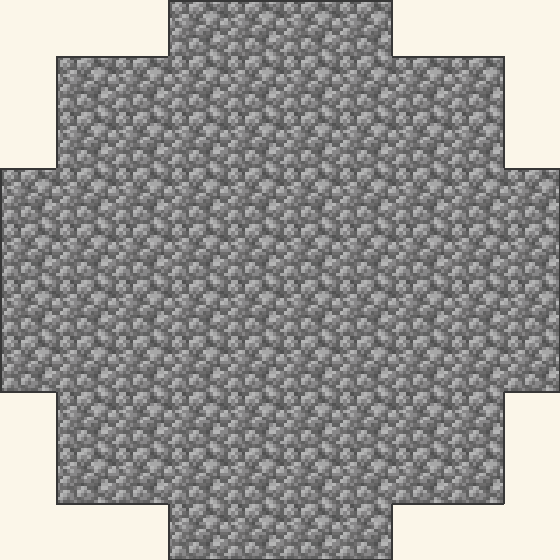
\includegraphics[width=\linewidth]{math_2d_d10_eucl.png}
  \caption{\emph{Euclidiano}}
\end{subfigure}\hfill
\begin{subfigure}[t]{0.30\linewidth}\centering
  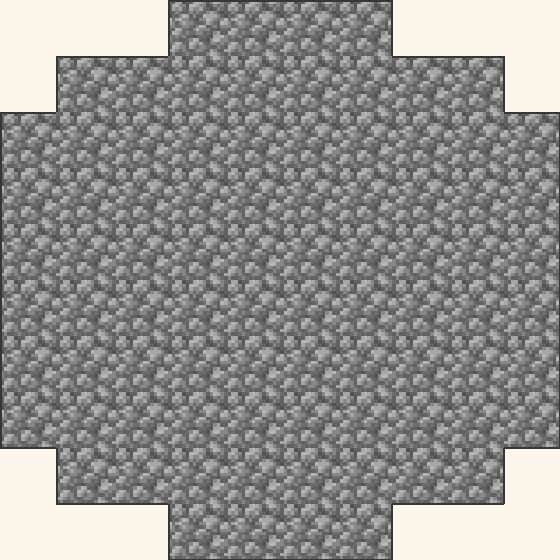
\includegraphics[width=\linewidth]{math_2d_d10_bres.png}
  \caption{\emph{Bresenham}}
\end{subfigure}\hfill
\begin{subfigure}[t]{0.30\linewidth}\centering
  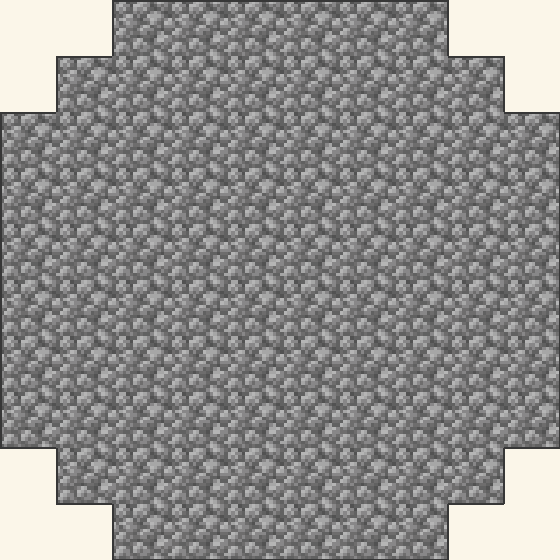
\includegraphics[width=\linewidth]{math_2d_d10_thr.png}
  \caption{\emph{Limiar}}
\end{subfigure}
\caption{Mesma circunferência de diâmetro $D=10$ sob os três critérios. Cada figura é o conjunto de células marcadas pela respectiva versão da desigualdade $d_x^2+d_y^2\leq 1$, renderizada com a textura \emph{cobblestone} do Minecraft. Note como a transição entre filas, as células de quina e os pontos cardeais variam --- três respostas matematicamente corretas sob critérios distintos.}
\label{fig:comp-d10}
\end{figure}

% =============================================================================
\section{Algoritmo Euclidiano (teste de distância)}

\textbf{Ideia.} Para cada linha $j$, encontre analiticamente as colunas $i$ que estão dentro da elipse. Resolvendo a equação da elipse para $x$, dado $y$:

\begin{formula}
\centering
$\displaystyle x \;=\; c_x \;\pm\; r_x\,\sqrt{\,1 - \left(\dfrac{y-c_y}{r_y}\right)^{\!2}\,}$
\end{formula}

Para uma linha $j$ cujo deslocamento vertical é $d_y = j+\tfrac{1}{2}-c_y$, a \emph{meia-largura horizontal} da elipse naquela altura é:

\begin{formula}
\centering
$\displaystyle \mathit{dxM} \;=\; r_x\,\sqrt{\,1 - \dfrac{d_y^{\,2}}{r_y^{\,2}}\,}$
\end{formula}

Se $d_y^{\,2}/r_y^{\,2} \geq 1$, a linha não intercepta a elipse e é pulada. Caso contrário, todas as colunas $i$ tais que $c_x - \mathit{dxM} \leq i+\tfrac{1}{2} \leq c_x + \mathit{dxM}$ são preenchidas. Os limites inteiros saem por:

\begin{formula}
\centering
$\displaystyle \mathit{lo} = \lceil c_x - \mathit{dxM} - \tfrac{1}{2} \rceil,
                \qquad
                \mathit{hi} = \lfloor c_x + \mathit{dxM} - \tfrac{1}{2} \rfloor$
\end{formula}

\textbf{Justificação.} O termo $+\tfrac{1}{2}$ resulta da convenção de que a célula de índice $i$ tem centro em $i+\tfrac{1}{2}$. As funções $\lceil\,\cdot\,\rceil$ e $\lfloor\,\cdot\,\rfloor$ realizam a conversão do intervalo contínuo para índices inteiros, garantindo que apenas células cujo \acc{centro} pertence ao interior da elipse sejam incluídas. Esta formulação produz a aproximação discreta mais próxima da curva contínua e, consequentemente, a silhueta de maior suavidade visual. Para diâmetros pequenos, contudo, o resultado pode apresentar menor caráter pixel-art em comparação aos demais --- um círculo Euclidiano com $D=5$ tem apenas $13$ blocos, enquanto o Limiar do mesmo diâmetro tem $21$.

\begin{minec}
\textbf{Mapeamento Minecraft.} O critério Euclidiano é o mais próximo do que o \cmd{//sphere} produz no WorldEdit. Para construir uma esfera de Pedra Lisa de $D=16$ ($r=8$) usando apenas a casca Euclidiana, o volume é $V \approx \tfrac{4}{3}\pi (8)^3 \approx 2\,145$ blocos no modo preenchido, caindo para aproximadamente $804$ blocos no modo fino (a casca) --- essa é a diferença entre coletar $34$ packs de Pedra Lisa ($34 \times 64 = 2\,176$) e $13$ packs ($13 \times 64 = 832$).
\end{minec}

% =============================================================================
\section{Algoritmo de Bresenham (ponto médio inteiro)}

O algoritmo de Bresenham, publicado em 1965 para o traçado de segmentos de reta, foi posteriormente estendido para circunferências e generalizado por Pitteway e Kappel para elipses arbitrárias. Sua propriedade distintiva é dispensar operações em ponto flutuante e extração de raiz quadrada: a determinação do próximo pixel utiliza exclusivamente \acc{somas e comparações sobre inteiros}, por meio de uma \emph{função de decisão} que avalia em qual lado da curva analítica se encontra o ponto médio entre os dois pixels candidatos. Para construção em Minecraft é o algoritmo que entrega o visual de pixel art mais \emph{reconhecível} --- a mesma silhueta escalonada que a comunidade tem construído manualmente desde 2011.

\subsection{Caso circular}

Para uma circunferência de raio inteiro $R$, parte-se de $(x{=}0,\,y{=}R)$ com parâmetro de decisão inicial:
\[
d_0 \;=\; 1 - R
\]

A cada passo (no octante de $0$ a $45°$):
\[
\begin{cases}
\text{se } d < 0: & \text{próximo é } (x{+}1,\;y), \quad d \mathrel{+}= 2x+3 \\[2pt]
\text{se } d \geq 0: & \text{próximo é } (x{+}1,\;y{-}1), \quad d \mathrel{+}= 2(x-y)+5
\end{cases}
\]

\textbf{Justificativa.} A função $d$ aproxima, a cada iteração, o valor da equação implícita da circunferência avaliada no \acc{ponto médio} entre as duas opções de pixel candidato:
\[
F\!\left(x+1,\;y-\tfrac{1}{2}\right) \;=\; (x+1)^2 + \left(y-\tfrac{1}{2}\right)^{\!2} - R^2
\]
O sinal de $d$ indica se o ponto médio se encontra no interior da circunferência (caso em que se avança apenas na horizontal) ou no exterior (caso em que se decrementa também a coordenada vertical). Os oito octantes da circunferência são obtidos por aplicação das simetrias do grupo diedral $D_4$ ao octante computado, o que corresponde, no código, às oito chamadas a \code{span(...)}. O traçado resultante exibe o padrão escalonado característico das aproximações discretas de curvas suaves --- e é precisamente a silhueta descrita nos tutoriais clássicos de pixel art Minecraft.

\subsection{Caso elíptico (duas regiões)}

Para uma elipse com semi-eixos $a, b$, o algoritmo divide o primeiro quadrante em \acc{duas regiões}, delimitadas pelo ponto onde a tangente faz $45°$:
\[
\text{Região I: } 2b^2 x < 2a^2 y \quad \bigl(|dy/dx| < 1\bigr),
\qquad
\text{Região II: caso contrário}
\]

Os parâmetros de decisão iniciais são:
\begin{align*}
p_1 &= b^2 - a^2 b + \tfrac{a^2}{4}, \\
p_2 &= b^2\!\left(x+\tfrac{1}{2}\right)^{\!2} + a^2\!\left(y-1\right)^{\!2} - a^2 b^2.
\end{align*}

Em cada iteração, $p$ é atualizado por incrementos pré-calculados (todos inteiros, após multiplicar por 4). O resultado é o mínimo de aritmética possível por pixel: \emph{um teste de sinal e duas somas}. O código usa \code{Math.floor} ao calcular $a$ e $b$ a partir de $r_x$ e $r_y$ para evitar adicionar uma linha extra fora do \emph{bounding-box} quando $r_y$ é não-inteiro.

\begin{minec}
\textbf{Mapeamento Minecraft.} Para construtores de survival a silhueta Bresenham costuma ser preferível à Euclidiana porque os passos discretos são mais fáceis de contar manualmente --- o usuário sabe que o próximo bloco é sempre \emph{reto} ou \emph{diagonal}, o que mantém o gesto consistente ao colocar. Um círculo Bresenham de $D=11$ tem a sequência canônica de $80$ blocos publicada em dezenas de guias da comunidade.
\end{minec}

% =============================================================================
\section{Algoritmo de Limiar (Threshold / cobertura de quina)}

Este algoritmo pergunta: \emph{existe alguma quina da célula que esteja dentro da elipse?} Para cada célula $(i,j)$, o código procura a quina mais próxima do centro da forma (projeção do centro nas arestas da célula):

\begin{formula}
\centering
$\displaystyle n_x = \operatorname{clamp}(c_x,\,i,\,i{+}1),\quad
                n_y = \operatorname{clamp}(c_y,\,j,\,j{+}1)$ \\[6pt]
$\displaystyle \text{dentro}\;\Longleftrightarrow\;
\left(\dfrac{n_x-c_x}{r_x}\right)^{\!2} + \left(\dfrac{n_y-c_y}{r_y}\right)^{\!2} \leq 0{,}94$
\end{formula}

O valor \acc{$0{,}94$} é um \emph{limiar empírico} ligeiramente inferior a $1{,}0$. Sua função é eliminar o artefato conhecido como \emph{spike tangencial} de 1 pixel, que ocorre nos quatro pontos cardeais (N, S, L, O), onde a curva é tangente a uma aresta inteira da célula. Sem essa redução, o algoritmo incluiria uma célula adicional cuja contribuição não melhora a representação visual da forma.

Entre os três algoritmos, este é o que produz a silhueta de maior área para um mesmo diâmetro $D$, uma vez que a condição de inclusão é a menos restritiva: basta que uma única quina da célula satisfaça a desigualdade da elipse para que a célula inteira seja preenchida. Para Minecraft, é o algoritmo que entrega o visual mais \emph{arredondado} ao custo de mais blocos --- $D=16$ produz $213$ blocos de casca sob Limiar contra $200$ sob Bresenham e $192$ sob Euclidiano.

\begin{minec}
\textbf{Mapeamento Minecraft.} Limiar é a escolha quando a construção será vista de longe (p.ex.\ uma cúpula de Quartzo sobre um templo), porque a silhueta levemente maior lê melhor através das sombras de oclusão ambiente. O trade-off é cerca de $5{-}10\%$ mais blocos por casca em relação à Euclidiana.
\end{minec}

% =============================================================================
\section{Modos de renderização: Preenchido, Fino, Grosso}

Tendo uma matriz $f[j][i] = 1$ para células internas, o projeto deriva três estilos visuais por \acc{topologia discreta}:

\subsection{Preenchido}
Retorna $f$ sem modificação. Todas as células internas viram blocos. É o que o \cmd{//sphere stone 8} produz.

\subsection{Fino (outline)}
Uma célula pertence ao contorno fino se está preenchida \emph{e} tem pelo menos um vizinho ortogonal (N, S, L, O) \emph{fora} da forma. Em notação lógica:
\[
b(i,j) \;=\; f(i,j) \;\wedge\;
\bigl(\neg f(i{-}1,j)\,\vee\,\neg f(i{+}1,j)\,\vee\,\neg f(i,j{-}1)\,\vee\,\neg f(i,j{+}1)\bigr)
\]
Geometricamente: é o \acc{bordo discreto} da forma, análogo discreto da fronteira topológica $\partial F = F \cap \overline{F^{\mathrm{c}}}$. Em Minecraft é o equivalente de \cmd{//hsphere} (esfera oca): só a casca é materializada.

\subsection{Grosso (thick)}
O modo grosso adiciona aos pixels de borda as \acc{pontes diagonais}: células internas que têm simultaneamente um vizinho-borda horizontal \emph{e} um vizinho-borda vertical. Isso preenche as \emph{células diagonais vazias} que o modo fino deixa entre os blocos da casca, útil quando o contorno precisa ser uma superfície contínua sem aberturas --- particularmente importante para cúpulas de Vidro e Gelo, onde cada célula diagonal vazia é, em Minecraft, um bloco de ar pelo qual água, monstros e luz transitam para o interior.
\begin{align*}
t(i,j) &= b(i,j) \;\vee\; \bigl(f(i,j) \,\wedge\, h_H \,\wedge\, h_V\bigr), \\
h_H &= b(i{-}1,j) \;\vee\; b(i{+}1,j), \\
h_V &= b(i,j{-}1) \;\vee\; b(i,j{+}1).
\end{align*}

\begin{minec}
\textbf{Mapeamento Minecraft.} Para uma cúpula de Vidro de $D=20$ (oca), o modo grosso produz uma casca \emph{contínua} de $608$ blocos contra $\approx 510$ blocos do modo fino --- os $\sim 100$ blocos extras são costura diagonal que elimina as células vazias deixadas a $45°$ pela voxelização, fechando o interior contra água, mobs e propagação de luz.
\end{minec}

\begin{figure}[!htbp]
\centering
\begin{subfigure}[t]{0.30\linewidth}\centering
  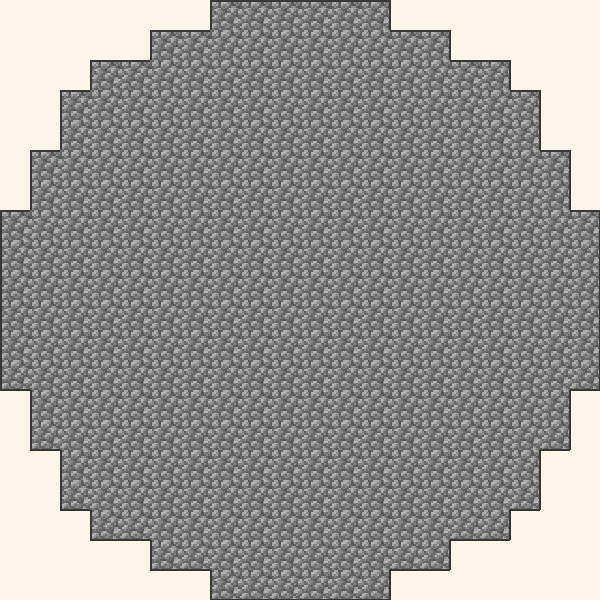
\includegraphics[width=\linewidth]{math_2d_d20_filled.png}
  \caption{\emph{Preenchido}}
\end{subfigure}\hfill
\begin{subfigure}[t]{0.30\linewidth}\centering
  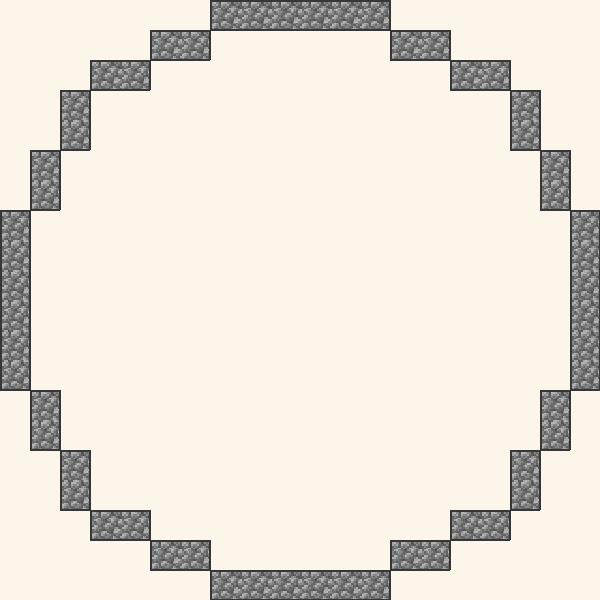
\includegraphics[width=\linewidth]{math_2d_d20_thin.png}
  \caption{\emph{Fino} (\emph{1 voxel})}
\end{subfigure}\hfill
\begin{subfigure}[t]{0.30\linewidth}\centering
  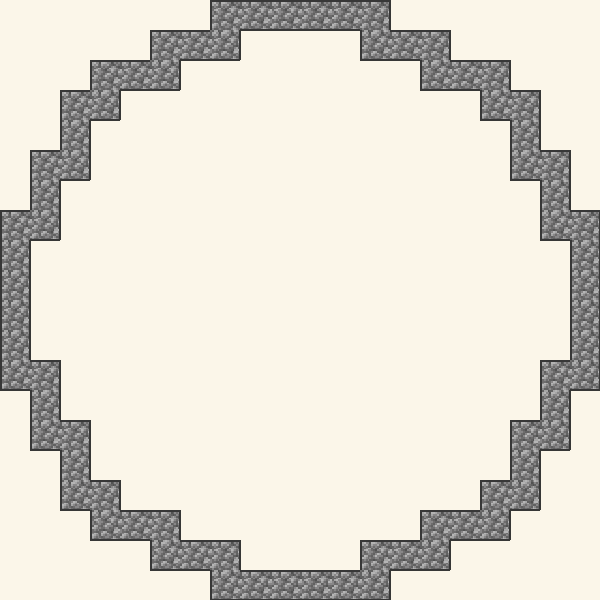
\includegraphics[width=\linewidth]{math_2d_d20_thick.png}
  \caption{\emph{Grosso}}
\end{subfigure}
\caption{Os três modos de renderização para a mesma circunferência euclidiana de $D=20$. O modo \emph{Fino} corresponde ao bordo discreto topológico ($\partial F$); o modo \emph{Grosso} adiciona blocos diagonais para fechar buracos a $45^\circ$, essencial para construções estanques (cúpulas de Vidro/Gelo subaquáticas).}
\label{fig:modes}
\end{figure}

% =============================================================================
\section{Cálculo de área discreta}

A função \code{area2D} simplesmente \acc{conta} as células marcadas em $f$. Isso é a \emph{medida de contagem}, que aproxima a integral de Riemann da função indicadora da elipse:
\[
\underset{\text{área contínua}}{\pi \, r_x \, r_y}
\qquad\longleftrightarrow\qquad
\underset{\text{área discreta}}{\sum_{j=0}^{G_y-1}\sum_{i=0}^{G_x-1} f(i,j)}
\]
Para $D$ grande, $\text{área discreta} / \text{área contínua} \to 1$. Para $D$ pequeno, a diferença entre algoritmos é visível: Limiar tende a superestimar; Euclidiano fica próximo da área ideal; Bresenham fica em algum lugar entre os dois.

\begin{minec}
\textbf{Mapeamento Minecraft.} O chip de contagem de blocos na UI do Block Round exibe exatamente esse número: $268$ para $D=8$, $904$ para $D=12$, $2\,145$ para $D=16$. O chip então expressa a contagem como \emph{$N$ (stacks $\times$ 64 + resto)} --- então $2\,145 = 33 \times 64 + 33$, ou seja, \enquote{$33$ stacks mais $33$ itens}, que é o que o usuário realmente precisa coletar.
\end{minec}

% =============================================================================
\section{Da 2D para 3D: a equação do elipsóide}

Em 3D, a forma fundamental é o \acc{elipsóide} centrado em $(c_x, c_y, c_z)$ com semi-eixos $r_x, r_y, r_z$. Sua equação é a generalização natural da elipse:
\[
\left(\dfrac{x}{r_x}\right)^{\!2} + \left(\dfrac{y}{r_y}\right)^{\!2} + \left(\dfrac{z}{r_z}\right)^{\!2} \;=\; 1
\]

Quando $r_x = r_y = r_z$, voltamos à \acc{esfera}. Avaliando no centro de cada voxel:
\[
a_\xi = \frac{\xi + \tfrac{1}{2} - c_\xi}{r_\xi}\;\;(\xi \in \{x,y,z\}),
\qquad
\text{dentro}\;\Longleftrightarrow\;a_x^{\,2} + a_y^{\,2} + a_z^{\,2} \leq 1
\]

\begin{minec}
\textbf{Mapeamento Minecraft.} Um elipsóide com $W=20$, $H=10$, $D=20$ produz uma \emph{esfera achatada} ideal para uma cúpula subterrânea ou um teto de estádio. O volume é $V = \tfrac{4}{3}\pi \cdot 10 \cdot 5 \cdot 10 \approx 2\,094$ blocos, equivalente a $33$ stacks de qualquer tipo de bloco. Comando WorldEdit equivalente: \cmd{//ellipsoid stone 10 5 10}.
\end{minec}

\begin{figure}[!htbp]
\centering
\begin{subfigure}[t]{0.46\linewidth}\centering
  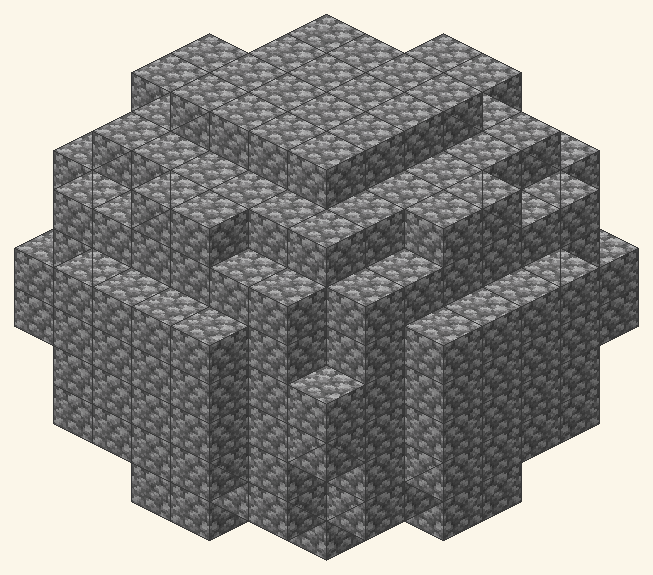
\includegraphics[width=\linewidth]{math_3d_sphere_d10.png}
  \caption{Esfera $D=10$, $r_x=r_y=r_z=5$.}
\end{subfigure}\hfill
\begin{subfigure}[t]{0.46\linewidth}\centering
  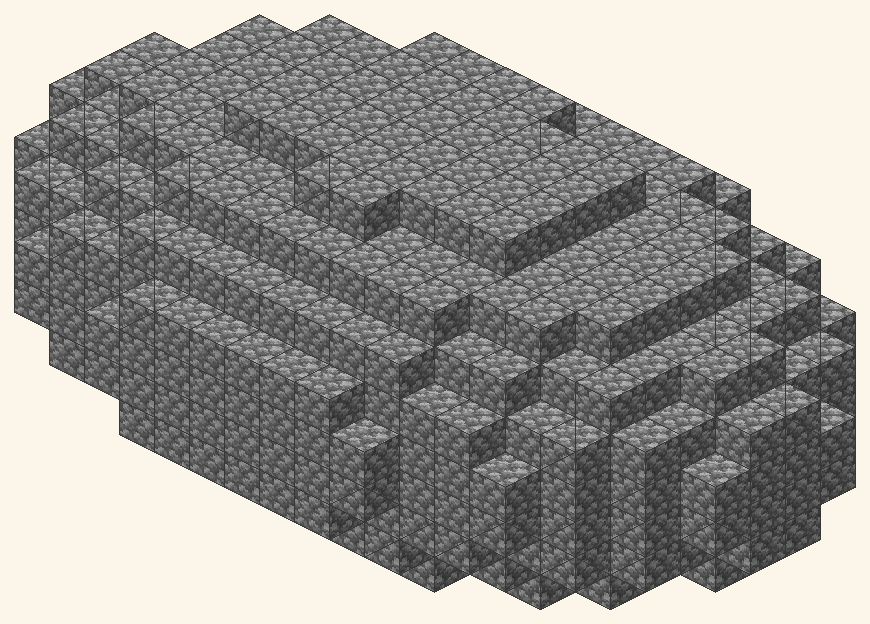
\includegraphics[width=\linewidth]{math_3d_ellipsoid.png}
  \caption{Elipsóide $W=20,\,H=10,\,D=12$.}
\end{subfigure}
\caption{Voxelização em $\mathbb{R}^3$. Cada cubo é um voxel; sua coordenada $(i,j,k)$ no centro é testada na equação implícita $a_x^2+a_y^2+a_z^2\leq 1$. As escadarias visíveis na superfície são consequência matemática da discretização --- exatamente o aspecto que dá ao Minecraft sua identidade visual.}
\label{fig:3d-shapes}
\end{figure}

% =============================================================================
\section{Voxelização e cálculo de volume}

O volume contínuo do elipsóide é um resultado clássico do cálculo integral, obtido por integração em discos:
\[
V \;=\; \dfrac{4}{3}\,\pi\, r_x\, r_y\, r_z
\]
A versão discreta percorre cada voxel da caixa $D_x \times D_y \times D_z$ e incrementa um contador quando $a_x^2 + a_y^2 + a_z^2 \leq 1$. Esse é o algoritmo de \code{voxelVolume}.

\textbf{Casca (shell) vs.\ interior.} Para o modo \emph{filled} o projeto mostra apenas os voxels com pelo menos um vizinho-6 fora do conjunto preservado (ou seja, voxels visíveis da superfície externa ou da face de corte). Para \emph{thin}, mostra apenas a \acc{superfície} do elipsóide completo (1 voxel de espessura). Em uma run de survival apenas as faces visíveis precisam receber seu bloco texturizado dedicado --- os voxels internos podem ficar com um bloco-bicho-papão barato (p.ex.\ Terra no lugar de Diamante) para economizar recursos.

\begin{minec}
\textbf{Tabela de referência.} A tabela abaixo resume os diâmetros canônicos de esfera mais pedidos pela comunidade Minecraft, traduzidos em número de blocos ($V$), packs de $64$ ($P=\lceil V/64\rceil$) e baús duplos de $54 \times 64 = 3\,456$ slots ($\mathrm{DC}=\lceil V/3{,}456 \rceil$). Use esta tabela para planejar a coleta de recursos antes da construção.
\end{minec}

\vspace{0.5em}
\begin{center}
\begin{tabular}{@{}lrrrr@{}}
\toprule
\textbf{Diâmetro} & \textbf{Blocos (V)} & \textbf{Packs (×64)} & \textbf{Baús duplos} & \textbf{Observação} \\
\midrule
D=8   &   268 &  5  & 1 & cúpula pequena  \\
D=12  &   904 & 15  & 1 & esfera média \\
D=16  &  2145 & 34  & 1 & topo de torre grande \\
D=20  &  4189 & 66  & 2 & teto de estádio \\
D=24  &  7238 & 114 & 3 & cúpula grande \\
D=32  & 17156 & 269 & 5 & mega-build \\
\bottomrule
\end{tabular}
\end{center}

Volumes em modo preenchido calculados sob o algoritmo Euclidiano em $D \in \{8,12,16,20,24,32\}$. Valores em modo fino (casca) são aproximadamente $V_{\mathrm{casca}} \approx 4\pi r^2 / 1$ bloco-espesso, ou seja, entre $25\%$ e $40\%$ do volume preenchido dependendo de $D$.

% =============================================================================
\section{Cortes geométricos: planos e o corte diagonal a $45°$}

O Block Round permite cortar o sólido por \acc{três planos}. Cada corte é uma \emph{desigualdade linear} que descarta voxels:
\[
\begin{array}{lcl}
\text{Eixo X:}    & x \geq \mathit{cut}      & \Rightarrow\; \text{descartado} \\
\text{Eixo Y:}    & y \geq \mathit{cut}      & \Rightarrow\; \text{descartado} \\
\text{Diagonal:}  & x + y \geq \mathit{cut}  & \Rightarrow\; \text{descartado}
\end{array}
\]

Os planos X e Y são perpendiculares aos eixos coordenados, com vetores normais $(1,0,0)$ e $(0,1,0)$. O \emph{plano diagonal} tem vetor normal $(1,1,0)/\sqrt{2}$ e corta a $45°$ no plano $XY$: matematicamente, é a família de planos $x+y = k$. Como o máximo de $x+y$ em uma caixa $D_x \times D_y$ vale $D_x + D_y$, o slider do corte diagonal tem amplitude $D_x + D_y$, enquanto X e Y têm amplitudes $D_x$ e $D_y$. O corte é \acc{proporcional}: o código guarda uma porcentagem $\mathit{cutPct}$ e recalcula o limite como
\[
\mathit{cut} \;=\; \mathit{cutPct} \cdot \max_{\text{eixo}}
\]
de modo que $50\%$ num eixo continua sendo $50\%$ quando o usuário troca de eixo ou redimensiona.

\begin{minec}
\textbf{Mapeamento Minecraft.} O corte no eixo Y a $50\%$ sobre uma esfera produz a clássica \emph{cúpula} de metade do volume. Para $D=16$: $V_{\mathrm{full}} = 2\,145$ blocos, $V_{\mathrm{cupula}} \approx 1\,095$ blocos ($\approx 18$ packs de $64$). O corte diagonal a $50\%$ produz uma seção \emph{meia-bacia} muito usada para interiores de fontes e arquibancadas de anfiteatro.
\end{minec}

\begin{figure}[!htbp]
\centering
\begin{subfigure}[t]{0.30\linewidth}\centering
  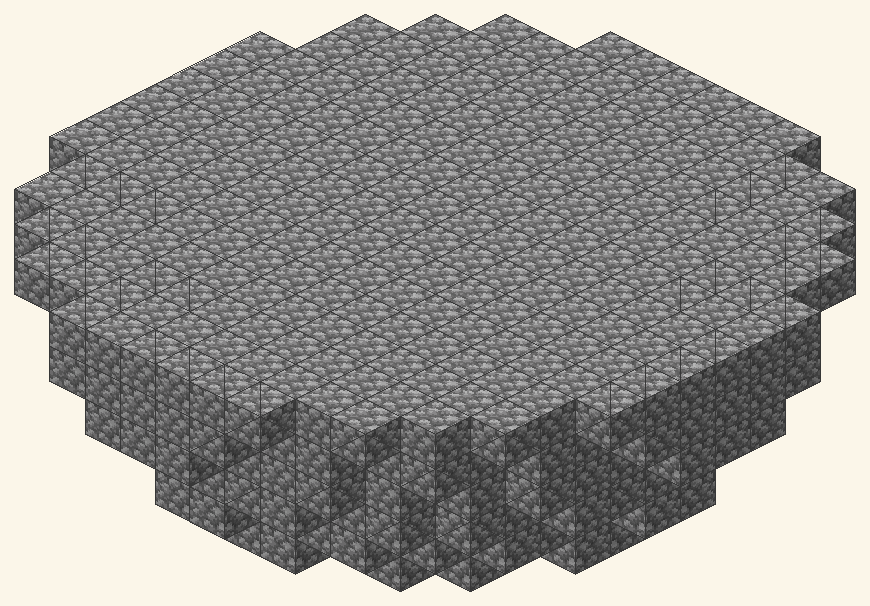
\includegraphics[width=\linewidth]{math_3d_cut_y.png}
  \caption{Corte $Y$ 50\% (cúpula)}
\end{subfigure}\hfill
\begin{subfigure}[t]{0.30\linewidth}\centering
  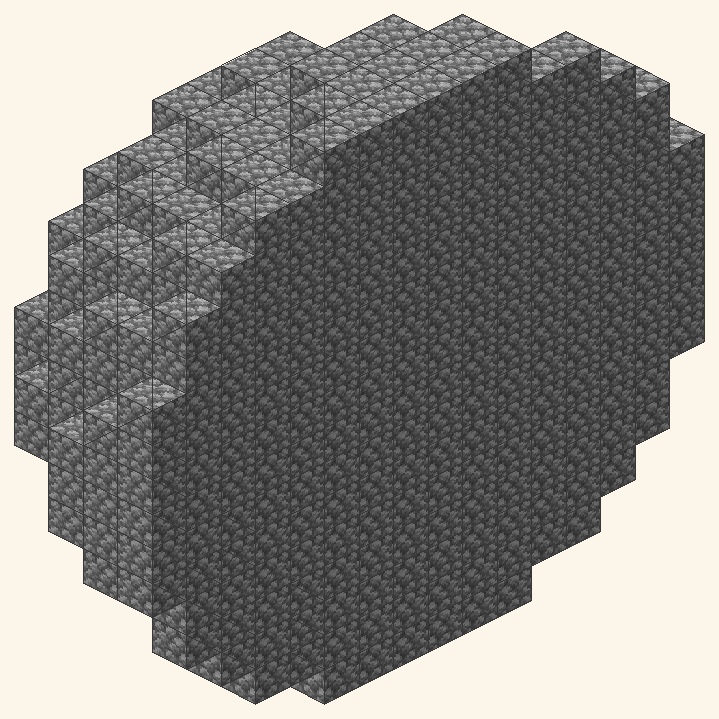
\includegraphics[width=\linewidth]{math_3d_cut_x.png}
  \caption{Corte $X$ 50\%}
\end{subfigure}\hfill
\begin{subfigure}[t]{0.30\linewidth}\centering
  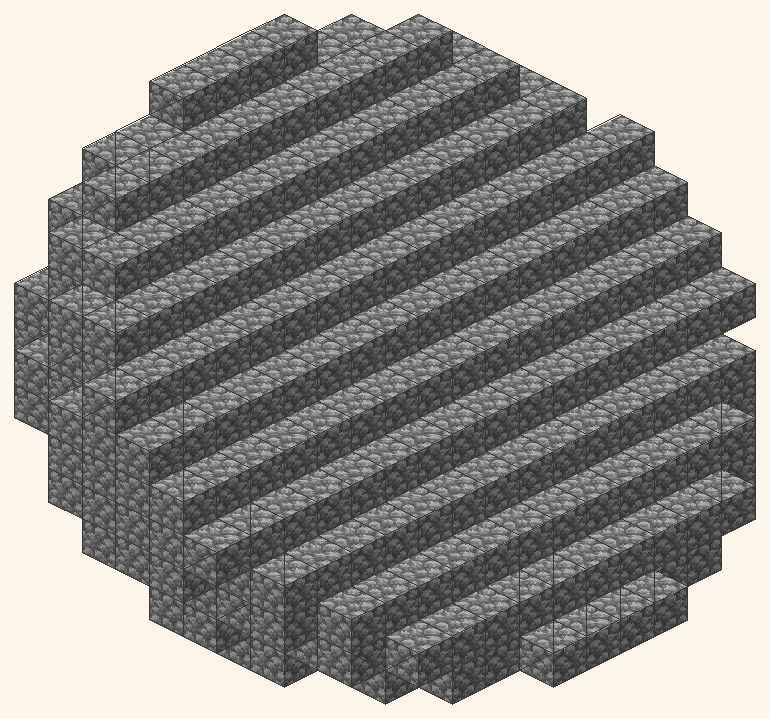
\includegraphics[width=\linewidth]{math_3d_cut_diag.png}
  \caption{Diagonal 50\%}
\end{subfigure}
\caption{Três cortes na mesma esfera $D=16$, todos preservando 50\% do volume. O corte $Y$ produz a cúpula clássica $V_{\mathrm{cúpula}}=\tfrac{2}{3}\pi r^3$; o diagonal expõe a hipotenusa $x+y=k$ característica desse plano de corte.}
\label{fig:cuts}
\end{figure}

% =============================================================================
\section{Modo Grosso 3D: tridimensionalização por fatias}

Para o modo \emph{thick} em 3D, o projeto aplica o algoritmo grosso 2D em \acc{todas as fatias} nos três eixos: $XY$ para cada $z$, $XZ$ para cada $y$, $YZ$ para cada $x$. Em seguida faz a \emph{união} dos resultados. A motivação geométrica é fechar a casca: o conjunto mínimo de voxels que preenchem todas as células diagonais vazias sem duplicar a espessura. Formalmente, sendo $S_z(z)$ a fatia $XY$ na altura $z$ e $T$ o operador grosso 2D:
\[
\mathit{thick3D} \;=\;
\bigcup_{z} T\bigl(S_z(z)\bigr) \;\cup\;
\bigcup_{y} T\bigl(S_y(y)\bigr) \;\cup\;
\bigcup_{x} T\bigl(S_x(x)\bigr)
\]
O resultado é depois interseccionado com o conjunto preservado pelo corte. A teoria por trás é \acc{topologia digital}: o operador grosso garante \emph{26-conectividade} da casca (vizinhos incluindo diagonais). Isso é relevante em Minecraft porque, mesmo que dois voxels da casca sejam vizinhos diagonais (compartilham só uma aresta), a célula entre eles continua sendo um bloco de ar pelo qual água e criaturas atravessam o interior --- o modo grosso fecha esses caminhos.

\begin{minec}
\textbf{Mapeamento Minecraft.} Para uma cúpula de Vidro subaquática sobre um monumento oceânico em survival, o modo grosso é obrigatório: as pontes diagonais preenchem as células vazias deixadas pelo modo fino, eliminando os caminhos de blocos-ar pelos quais a água invadiria. Custo: cúpula de $D=20$ em modo grosso exige $\approx 380$ blocos de Vidro contra $\approx 320$ em modo fino --- $19\%$ a mais de material em troca de uma casca completamente fechada.
\end{minec}

% =============================================================================
\section{Câmera 3D: coordenadas esféricas}

A câmera 3D orbita o objeto a uma distância $r$ com dois ângulos --- $\theta$ (azimute, no plano horizontal) e $\varphi$ (polar, do eixo vertical). Essa é a \acc{convenção física} de coordenadas esféricas, e a conversão para cartesianas (a forma que \emph{three.js} entende) é:
\[
\begin{aligned}
x &= r\,\sin(\varphi)\,\cos(\theta), \\
y &= r\,\cos(\varphi), \\
z &= r\,\sin(\varphi)\,\sin(\theta).
\end{aligned}
\]
Posição inicial: $\theta = \pi/4$ ($45°$, perspectiva isométrica) e $\varphi = \pi/3$ ($60°$ a partir do polo Norte, levemente acima do equador). Arrasto do mouse incrementa $\theta$ e $\varphi$ diretamente; roda/pinça incrementa $r$. A simplicidade dessa parametrização é o que permite a rotação livre sem nenhum quatérnio ou matriz explícita.

% =============================================================================
\section{Auto-zoom: esfera envolvente e FOV}

Quando o usuário muda o tamanho da figura ou reseta a câmera, o projeto recalcula a \acc{distância ideal} da câmera para que o objeto caiba na tela em qualquer ângulo. A ideia é encerrar o objeto numa \emph{esfera de raio $R$} (a metade da diagonal da AABB, axis-aligned bounding box):
\[
R \;=\; \sqrt{\,(D_x/2)^2 + (D_y/2)^2 + (D_z/2)^2\,}
\]

Uma esfera tem \acc{projeção invariante por rotação}, então se ela couber na tela em uma orientação, cabe em todas. Dado o FOV vertical da câmera ($\mathit{fov}_V = 35°$ em radianos), a distância necessária para enquadrar uma esfera de raio $R$ é:
\[
\mathit{dist}_V \;=\; \dfrac{R}{\tan(\mathit{fov}_V / 2)}
\]
O FOV horizontal sai da razão de aspecto do canvas ($\mathit{aspect} = \text{largura}/\text{altura}$) por:
\[
\mathit{fov}_H \;=\; 2\,\arctan\!\left(\,\tan(\mathit{fov}_V/2)\cdot \mathit{aspect}\,\right)
\]
A distância final é o máximo entre $\mathit{dist}_V$ e $\mathit{dist}_H$, multiplicado por $1{,}20$ ($20\%$ de margem visual). Quando a figura está cortada, o código encolhe $D_x$ ou $D_y$ para o tamanho restante, de modo que uma esfera cortada a $75\%$ não apareça minúscula no canto. Quando o easter egg da árvore de carvalho ou do creeper está ativo, o bounding box é estendido para cima para incluir a altura da entidade.

% =============================================================================
\section{Tons (shading) e multiplicação de textura}

Os três estilos 3D (\emph{Classic}, \emph{Smooth}, \emph{Blocks}) diferenciam-se por \acc{fatores multiplicativos} aplicados às três faces visíveis de cada voxel (topo, lado iluminado, lado escuro). A função \code{shadeHex(hex, factor)} parseia o hex em $(R,G,B)$ e multiplica cada canal, com \emph{clamp} em $[0, 255]$ --- e o resultado vira um tint aplicado sobre a textura crua do bloco:
\[
R' = \mathrm{clamp}(R \cdot f),\quad
G' = \mathrm{clamp}(G \cdot f),\quad
B' = \mathrm{clamp}(B \cdot f)
\]
Isso é uma \emph{aproximação linear} da função de iluminação Lambertiana ideal,
\[
I \;=\; \max\bigl(0,\;\mathbf{n}\cdot\mathbf{l}\bigr)\cdot \mathit{textura},
\]
quando os três fatores correspondem ao cosseno do ângulo entre a normal de cada face e a direção de luz fixa. Em \emph{Smooth} os fatores são próximos (faces parecidas); em \emph{Classic} os fatores diferem mais (contraste forte, o visual do Minecraft vanilla). \emph{Blocks} ainda introduz uma reentrância geométrica nos voxels --- uma translação constante de cada face para dentro, para revelar as fronteiras entre voxels mesmo quando vizinhos têm a mesma textura. Para blocos emissivos (Glowstone, Sea Lantern, Shroomlight, Magma, Crying Obsidian) o termo Lambertiano é substituído por uma constante $I = \mathit{fator\_emissivo} \cdot \mathit{textura}$ escalada pelo nível de luz do bloco no MC.

\begin{figure}[!htbp]
\centering
\begin{subfigure}[t]{0.30\linewidth}\centering
  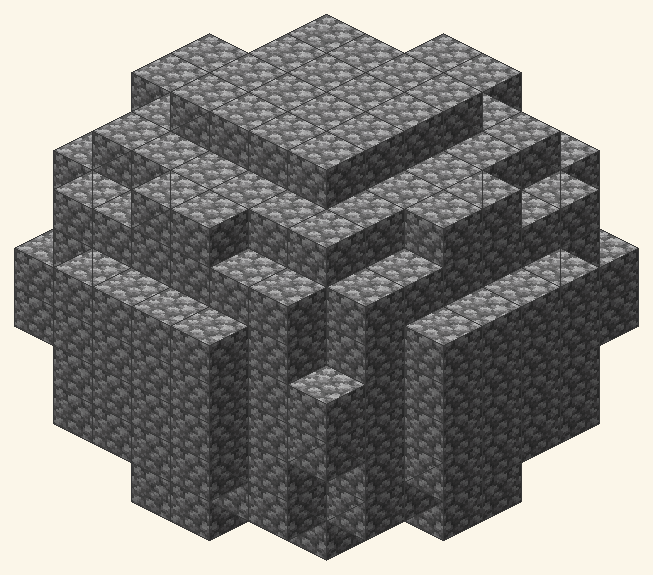
\includegraphics[width=\linewidth]{math_3d_shading_classic.png}
  \caption{\emph{Classic} (contraste forte)}
\end{subfigure}\hfill
\begin{subfigure}[t]{0.30\linewidth}\centering
  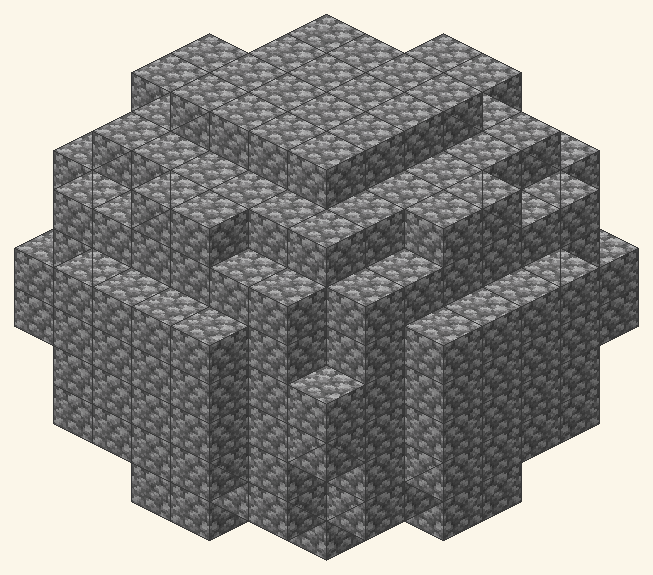
\includegraphics[width=\linewidth]{math_3d_shading_blocks.png}
  \caption{\emph{Blocks} (default)}
\end{subfigure}\hfill
\begin{subfigure}[t]{0.30\linewidth}\centering
  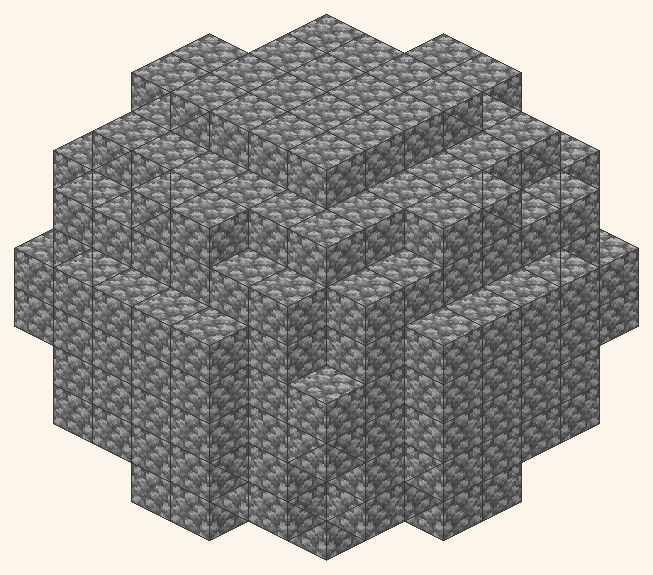
\includegraphics[width=\linewidth]{math_3d_shading_smooth.png}
  \caption{\emph{Smooth} (faces parecidas)}
\end{subfigure}
\caption{Três multiplicadores de luz aplicados às mesmas três faces visíveis. \emph{Classic} dá o aspecto canônico Minecraft vanilla; \emph{Smooth} reduz o contraste para superfícies suaves; \emph{Blocks} é o intermediário com inset geométrico que revela fronteiras entre voxels mesmo quando a textura é a mesma.}
\label{fig:shading}
\end{figure}

% =============================================================================
\section{Transição: da matemática contínua para a construção no jogo}

As quinze seções acima descrevem o pipeline \emph{contínuo-para-discreto} que o Block Round compartilha com o projeto-irmão Pixel Round: da equação implícita da elipse até a câmera que enquadra o resultado. As seis seções restantes descrevem o que é \acc{específico} ao Block Round --- a camada adicional de matemática introduzida pelo fato de que as células renderizadas não são pixels abstratos, mas \emph{blocos de Minecraft}, cada um com seis faces texturizadas, um peso no inventário e um custo de tempo para coletar e colocar.

Não são considerações cosméticas. A decisão de renderizar com texturas de blocos muda o problema operacional do usuário: em vez de \emph{exportar um PNG}, o usuário precisa \emph{traduzir a silhueta em um plano de colocação}. O conteúdo matemático das próximas seções trata exatamente dessa tradução: aritmética de inventário, otimização de contagem de faces, decomposição camada-por-camada, e exploração de simetria para reduzir o custo de $N$ colocações para $N/8 + 7$ invocações de comando.

\clearpage

% =============================================================================
\section{Aritmética do inventário Minecraft}

Um jogador de Minecraft carrega itens num \emph{inventário} de 36 slots organizados como uma grade $9 \times 4$. Cada slot suporta no máximo $64$ itens do mesmo tipo (uma \emph{stack} ou \emph{pack}). O jogador também acessa \emph{armazenamento}: um baú simples tem $27$ slots, um baú duplo tem $54$ slots. A aritmética que traduz um número-alvo de blocos em um plano de coleta é, portanto, um problema de \emph{divisão com teto}.

\subsection{Slot único, stack única, pack cheio}
O \emph{stack} é a unidade elementar de contabilidade de inventário. Cada stack contém no máximo $64$ itens. A conversão da contagem de blocos $N$ em packs (ou stacks) é

\subsection{Armazenamento: baús, baús duplos, shulker boxes}
Para calcular quantos \emph{baús duplos} uma construção exige, divida a contagem de blocos pelos $54$ slots $\times$ $64$ itens/slot $= 3\,456$ itens por baú duplo:
\[
\text{packs}:\quad N_{\mathrm{packs}} \;=\; \left\lceil \dfrac{N}{64} \right\rceil
\qquad
\text{baús duplos}:\quad N_{\mathrm{dc}} \;=\; \left\lceil \dfrac{N}{3456} \right\rceil
\]
Um \emph{baú simples} guarda $27 \times 64 = 1\,728$ itens. Uma \emph{shulker box} (container portátil) guarda $27 \times 64 = 1\,728$ itens mas pode ela mesma ser guardada \emph{dentro} de um slot de baú, então um baú duplo cheio de $54$ shulker boxes guarda até $54 \times 1\,728 = 93\,312$ itens. Para mega-builds a unidade de capacidade relevante é o \emph{baú duplo carregado de shulkers}.

\subsection{Tabela de referência: esferas canônicas}
A tabela abaixo converte os volumes canônicos de esfera preenchida em planos de coleta. A última coluna sugere um contexto de construção para cada diâmetro:

\vspace{0.4em}
\begin{center}
\small
\begin{tabularx}{\textwidth}{@{}lrrlX@{}}
\toprule
\textbf{Diâmetro} & \textbf{V (blocos)} & \textbf{Packs} & \textbf{Armazenamento} & \textbf{Construção típica} \\
\midrule
D=8   &   268 &  5  &  1 bd & telhado de cabana, cúpula de poço  \\
D=12  &   904 & 15  &  1 bd & topo de torre de vigia \\
D=16  &  2145 & 34  &  1 bd & sino de aldeão, cúpula de biblioteca \\
D=20  &  4189 & 66  &  2 bds & cúpula de observatório \\
D=24  &  7238 & 114 &  3 bds & cúpula de templo \\
D=32  & 17156 & 269 &  5 bds & cúpula de catedral, arena de world-boss \\
\bottomrule
\end{tabularx}
\end{center}

A representação \emph{stacks-e-resto} $N = q \cdot 64 + r$ exibida pelo chip de info do Block Round espelha a forma como o inventário de survival exibe stacks parciais: o jogador vê $q$ slots cheios mais um slot mostrando $r$. Para $D=16$, o chip imprime \enquote{$2\,145$ ($33 \times 64 + 33$)}, dizendo ao jogador para preencher $33$ slots completamente mais um slot com $33$ itens --- exatamente $34$ slots, o que cabe numa única fileira do inventário mais quatro slots extras.

% =============================================================================
\section{Highlight overlay e contagem de faces expostas}

O Block Round renderiza, por padrão, um \emph{contorno preto} (highlight overlay) nas arestas de cada face de voxel visível. Visualmente isso lembra o estilo \enquote{F3+G} de fronteira de chunk do overlay de debug do jogo, mas escalado para o nível por-voxel. Matematicamente o overlay implementa a visualização da \acc{contagem de faces expostas}: um número que construtores de survival usam para validar progresso bloco-a-bloco.

\subsection{O que conta como face exposta}
Uma face do voxel $\mathbf{v}$ compartilhada com o vizinho $\mathbf{n}$ é \emph{exposta} se e somente se $\mathbf{n} \notin V_{\mathrm{sólido}}$ (o vizinho é vazio). Cada voxel sólido contribui entre $0$ (totalmente enterrado, interno ao sólido) e $6$ (isolado) faces. A contagem total de faces expostas $F_{\mathrm{exp}}$ é o análogo discreto da \emph{área de superfície} da figura.

\subsection{Fórmula de detecção de bordo}
Um voxel está no bordo se pelo menos um de seus seis vizinhos-por-face está fora do sólido:
\[
b(i,j,k) \;=\; f(i,j,k) \;\wedge\; \bigl(\neg f(i{\pm}1,j,k)\,\vee\,\neg f(i,j{\pm}1,k)\,\vee\,\neg f(i,j,k{\pm}1)\bigr)
\]
É o mesmo operador de bordo do algoritmo fino 2D estendido para 3D, e o highlight overlay simplesmente desenha as linhas de aresta cúbicas de cada voxel-bordo. Para Vidro e Gelo o padrão é OFF, já que os frames com alpha-blending já fazem o trabalho; para Pedra Lisa, Pedra, Diamante e outros blocos opacos o padrão é ON, porque o overlay desambigua voxels internos da casca.

\subsection{Contagem de faces expostas como heurística de survival}
Para construtores de survival a contagem relevante não é o volume total $V$ mas a \emph{contagem de faces expostas} $F_{\mathrm{exp}}$, porque é isso que é visível de fora. O total $F_{\mathrm{exp}}$ sobre todos os voxels sólidos é igual a seis vezes a contagem de voxels-bordo menos duas vezes o número de adjacências-face entre voxels-bordo:
\[
F_{\mathrm{exp}} \;=\; \sum_{\mathbf{v}\in V_{\mathrm{solid}}}\;\sum_{\mathbf{n}\in N_6(\mathbf{v})}\!\!\bigl[\mathbf{v}+\mathbf{n}\notin V_{\mathrm{solid}}\bigr]
\]
Para uma esfera de $D=16$ (modo preenchido), $V = 2\,145$, $V_{\mathrm{bordo}} \approx 432$ (a casca), e $F_{\mathrm{exp}} \approx 1\,184$ faces visíveis --- ou seja, a construção precisa de apenas cerca de $432$ blocos \emph{visíveis}; os $1\,713$ restantes são interior e podem ser preenchidos com o bloco mais barato disponível (Terra, Pedra Lisa). O highlight overlay permite ao construtor identificar imediatamente um bloco faltante na casca, porque um voxel ausente produz uma descontinuidade no padrão do overlay que o olho capta de relance.

\begin{figure}[!htbp]
\centering
\begin{subfigure}[t]{0.40\linewidth}\centering
  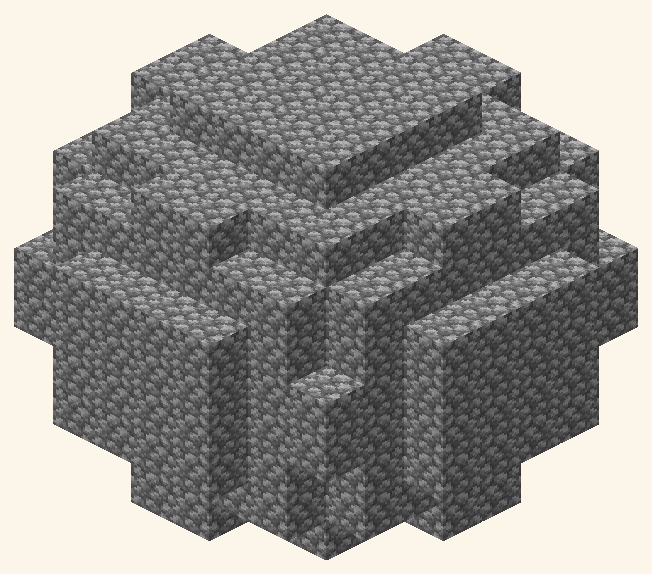
\includegraphics[width=\linewidth]{math_3d_overlay_off.png}
  \caption{Overlay \emph{OFF}}
\end{subfigure}\hfill
\begin{subfigure}[t]{0.40\linewidth}\centering
  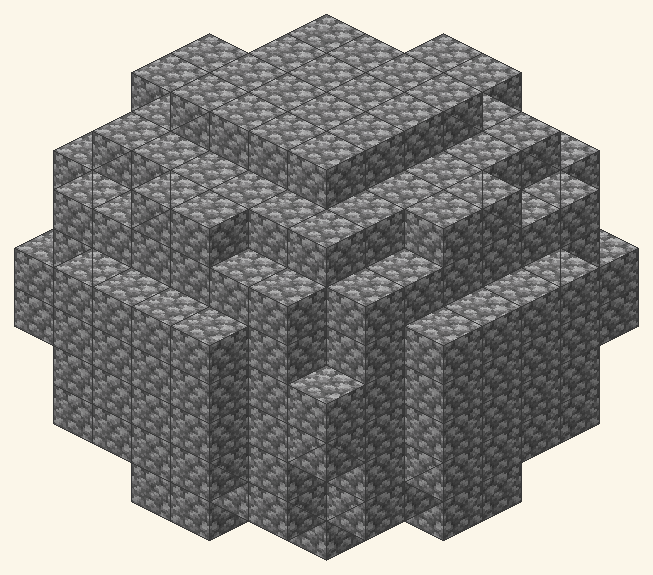
\includegraphics[width=\linewidth]{math_3d_overlay_on.png}
  \caption{Overlay \emph{ON} (default)}
\end{subfigure}
\caption{Mesmo conjunto de voxels com e sem o contorno preto nas arestas expostas. Com o \emph{highlight overlay} ON, um bloco faltante na casca produz uma descontinuidade no padrão que o olho detecta de relance --- ferramenta de validação rápida durante a construção em survival.}
\label{fig:overlay}
\end{figure}

% =============================================================================
\section{Construção camada-por-camada (decomposição horizontal)}

No Minecraft a construção avança \emph{por camadas horizontais}: o jogador fica em pé numa camada, coloca os blocos da camada acima, depois sobe um bloco (pula + coloca andaime temporário ou usa elytra). O problema do elipsóide 3D, portanto, é melhor entendido como uma \emph{pilha de elipses 2D}, uma por camada:
\[
\text{\text{camada}(k)} \;=\; \bigl\{\,(i,j)\;:\;a_x(i)^2 + a_y(j)^2 \leq 1 - a_z(k)^2\,\bigr\}
\]

Para cada camada inteira $k$ de $-r_z$ até $+r_z$, a secção transversal é ela mesma uma elipse com semi-eixos encolhidos $r_x(k)$ e $r_y(k)$:
\[
r_x(k) \;=\; r_x\,\sqrt{\,1 - \left(\dfrac{k}{r_z}\right)^{\!2}\,},
\qquad
r_y(k) \;=\; r_y\,\sqrt{\,1 - \left(\dfrac{k}{r_z}\right)^{\!2}\,}
\]
Isso quer dizer que o problema 3D se reduz a \emph{calcular o algoritmo 2D das seções anteriores, uma camada por vez}, e empilhar os resultados. Cognitivamente é uma simplificação enorme: em vez de rastrear três coordenadas mentalmente, o construtor rastreia duas coordenadas por camada mais o índice da camada. Cada camada vira um problema 2D já resolvido pelos algoritmos das Seções~4--6.

\begin{minec}
\textbf{Mapeamento Minecraft.} Para uma esfera de $D=16$ ($r_z = 8$), a camada equatorial ($k=0$) é o círculo Bresenham $D=16$ completo ($\approx 200$ blocos). A próxima camada acima ($k=1$) é um círculo $D=15{,}97$, essencialmente a mesma forma menos as células de quina. Em $k=4$ a camada é um círculo $D=13{,}86$ (cerca de $148$ blocos), e em $k=7$ encolheu para um círculo $D=7{,}48$ (cerca de $43$ blocos). Os polos ($k = \pm 8$) são uma tampa de um bloco.
\end{minec}

O chip de info do Block Round expõe essa contagem por camada em modo 3D quando o usuário ativa o botão de Guides centrais (tecla \code{C}). As fatias horizontais são desenhadas como uma cruz amarela translúcida no equador e em cada subdivisão $r_z/2$, dando ao construtor uma referência clara de onde caem as fronteiras de camada.

% =============================================================================
\section{Otimização via simetria octaédrica ($O_h$)}

Uma esfera centrada na origem é invariante sob a ação do \acc{grupo octaédrico} $O_h$ de ordem $48$. A voxelização da esfera preserva um subgrupo de ordem $48$ gerado pelas três reflexões coordenadas e pelas três rotações de $\pi/2$ ao redor de cada eixo. Para fins práticos de construção, o subgrupo relevante é o grupo de reflexões octaédricas $\mathbb{Z}_2^3$ de ordem $8$, gerado por $x \mapsto -x$, $y \mapsto -y$, $z \mapsto -z$. O conjunto de voxels num octante determina a esfera inteira:
\[
V_{\mathrm{total}} \;\approx\; 8\,V_{\mathrm{octant}}\;\;\Longrightarrow\;\;
\text{redução}\;=\;\frac{N - N/8}{N} \;=\; 87{,}5\%
\]

Essa é a maior otimização matemática disponível para um construtor de Minecraft. Em vez de colocar manualmente $N$ blocos, o construtor coloca $N/8$ blocos no octante positivo e depois emite sete comandos \cmd{/clone} (vanilla) ou \cmd{//copy + //paste} (WorldEdit) com as reflexões apropriadas.

\subsection{Sequência concreta de comandos}
Para uma esfera de $D=24$ ($r=12$, $V = 7\,238$ blocos) centrada nas coordenadas-mundo $(0,72,0)$, construa o octante positivo primeiro (a região $+x, +y, +z$, $\approx 905$ blocos), depois emita:

\begin{minec}
\cmd{/clone 0 72 0 12 84 12 \textasciitilde\,\textasciitilde\,\textasciitilde\ filtered minecraft:stone}\\
\cmd{/clone 0 72 0 12 84 12 -12 72 0 mode:masked} \quad (reflex.\ \(-x\))\\
\cmd{/clone 0 72 0 12 84 12 0 60 0 mode:masked} \quad\quad (reflex.\ \(-y\))\\
\cmd{/clone 0 72 0 12 84 12 0 72 -12 mode:masked} \quad (reflex.\ \(-z\))\\
\cmd{/clone -12 72 0 -1 84 12 mode:masked} \quad\quad\quad\;\; (octante \(-x,-y\))\\
\cmd{/clone 0 60 -12 12 71 -1 mode:masked} \quad\quad\quad (octante \(-y,-z\))\\
\cmd{/clone -12 72 -12 -1 84 -1 mode:masked} \quad\;\; (octante \(-x,-z\))\\
\cmd{/clone -12 60 -12 -1 71 -1 mode:masked} \quad\;\; (octante \(-x,-y,-z\))
\end{minec}

Cada \cmd{/clone} custa cerca de $50$\,ms de tempo de servidor, então as sete reflexões completam em menos de meio segundo. A colocação manual dos $905$ blocos do octante leva cerca de $15$\,min em survival ou $45$\,s em creative com brush. A colocação completa de $7\,238$ blocos (sem simetria) levaria $\approx 2$\,h em survival ou $6$\,min em creative.

\subsection{Comparação de tempo}
Seja $T_{\mathrm{block}}$ o tempo de colocação por bloco (tipicamente $1{-}2$\,s em survival, $0{,}1{-}0{,}5$\,s em creative) e $T_{\mathrm{clone}}$ o tempo do comando por clone ($\approx 50$\,ms). O tempo total de construção com e sem simetria é:
\[
T_{\mathrm{octant}} \;+\; 7\,T_{\mathrm{clone}}
\quad\ll\quad
T_{\mathrm{full}}
\]
Para $N = 7\,238$ em survival ($T_{\mathrm{block}} = 2$\,s, $T_{\mathrm{clone}} = 0{,}05$\,s): cheio = $14\,476$\,s $\approx 4$\,h $1$\,min; octante + clones = $1\,810$\,s + $0{,}35$\,s $\approx 30$\,min. Um fator-$8$ de aceleração que casa exatamente com a ordem do subgrupo de reflexões. O grupo octaédrico completo $O_h$ de ordem $48$ poderia em princípio reduzir mais ainda (por um fator de $48$), mas explorar as rotações diagonais exige uma área rotada a $45°$, o que raramente vale o custo de setup no Minecraft vanilla.

\begin{figure}[!htbp]
\centering
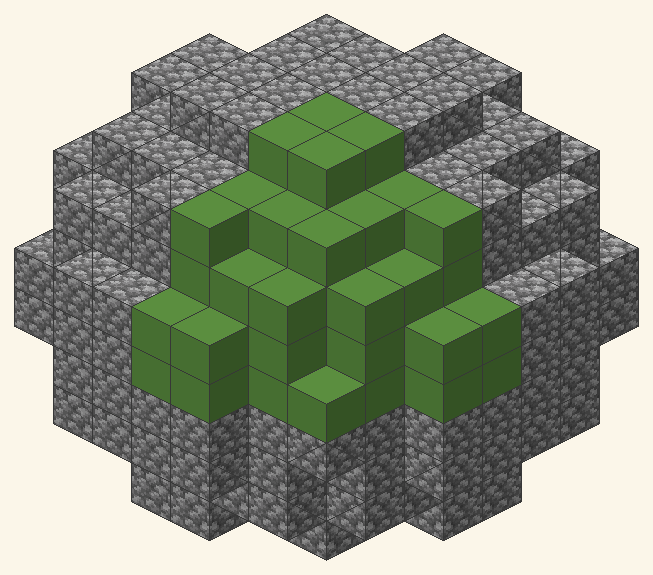
\includegraphics[width=0.45\linewidth]{math_3d_octants.png}
\caption{Esfera $D=10$ com o octante positivo $(+x,+y,+z)$ destacado em verde. Sob a ação do subgrupo $\mathbb{Z}_2^3 \leq O_h$ (ordem 8, gerado pelas três reflexões coordenadas), esse octante determina toda a esfera --- as outras sete regiões são obtidas por uma sequência de \cmd{/clone} com \emph{mode:masked} aplicadas sobre o octante construído manualmente.}
\label{fig:octants}
\end{figure}

% =============================================================================
\section{Texturas de bloco e composição visual}

Um bloco de Minecraft não é uma célula plana e colorida, mas um \emph{cubo com seis faces texturizadas}. O Block Round renderiza cada voxel com suas seis texturas canônicas de face, amostradas do resource pack vanilla. Matematicamente a operação de texturização é um \emph{mapeamento UV}: cada face do cubo unitário é parametrizada por coordenadas $[0,1]^2$, e a textura correspondente é amostrada nessas UVs para produzir os pixels renderizados.

\subsection{As seis faces e o mapeamento UV}
Para cada face de voxel o renderer consulta o modelo do bloco:
\[
\text{face}\;\in\;\{\,\text{topo},\;\text{lado},\;\text{fundo}\,\}
\qquad
\mathrm{UV}: [0,1]^2 \to \text{pixels}
\]

A maioria dos blocos (Pedra, Pedra Lisa, Bloco de Diamante, Tábuas de Carvalho) usa a \emph{mesma textura em todas as seis faces}. Blocos multi-face (Bloco de Grama, Abóbora, Fardo de Feno, Pilar de Quartzo, todos os troncos de árvore, Bancada, Fornalha, Estante, TNT) usam \emph{texturas diferentes} no topo, nos lados e no fundo: Bloco de Grama tem topo verde, lado grama-com-terra e fundo terra puro; um Tronco de Carvalho tem o anel da madeira no topo/fundo e a casca nas quatro laterais. Crucialmente a \emph{matemática de quais voxels colocar} não depende da textura usada --- a silhueta de uma esfera de Diamante e a de uma esfera de Pedra Lisa do mesmo diâmetro é idêntica. A decisão de textura é uma camada \emph{puramente estética} aplicada depois do algoritmo geométrico terminar.

\subsection{Famílias de blocos e tonalidades}
Para o construtor de survival escolhendo entre as dezenas de blocos disponíveis, a pergunta relevante não é o índice da textura mas a \emph{família tonal}: claro/escuro, quente/frio, uniforme/padronizado. A tabela abaixo classifica os blocos mais usados em construções no Block Round:

\vspace{0.4em}
\begin{center}
\begin{tabular}{@{}llll@{}}
\toprule
\textbf{Bloco} & \textbf{Família} & \textbf{Tom} & \textbf{Uso típico} \\
\midrule
cobblestone        & pedra  & cinza  & muros rústicos, masmorras \\
stone              & pedra  & cinza  & muros limpos, pedestais \\
oak\_planks        & madeira   & bege   & pisos, acabamento interno \\
quartz\_block      & quartzo    & branco   & templos, cúpulas modernas \\
sandstone          & areia   & bege   & desertos, pirâmides \\
deepslate          & pedra  & escuro  & subterrâneos, acentos \\
\bottomrule
\end{tabular}
\end{center}

\subsection{Gradientes via mistura de blocos}
Embora um único tipo de bloco entregue um tom, \emph{gradientes} podem ser obtidos intercalando dois ou três tipos por camada. Uma técnica clássica é o gradiente \emph{pedra-para-quartzo} numa cúpula: as camadas de baixo são Pedra Lisa, as camadas equatoriais são uma mistura ruidosa de Pedra Lisa e Diorito, e as camadas de cima são Quartzo. Cada camada continua calculada pelo mesmo algoritmo do Block Round; o que muda é o lookup de textura por voxel. A opção de bloco \emph{Random} do Block Round implementa uma mistura procedural desse tipo por padrão (tampa de grama, terra logo abaixo, minérios esparsos no meio, deepslate perto da bedrock). A matemática é a mesma da decomposição por camada da Seção~19; só a \enquote{tag de bloco} por voxel muda.

\begin{figure}[!htbp]
\centering
\begin{subfigure}[t]{0.30\linewidth}\centering
  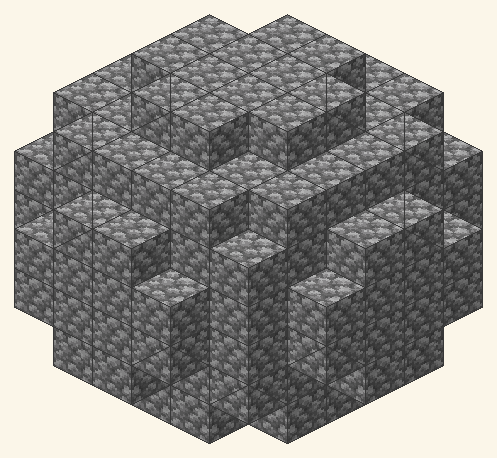
\includegraphics[width=\linewidth]{math_3d_tex_cobble.png}
  \caption{\emph{Cobblestone}}
\end{subfigure}\hfill
\begin{subfigure}[t]{0.30\linewidth}\centering
  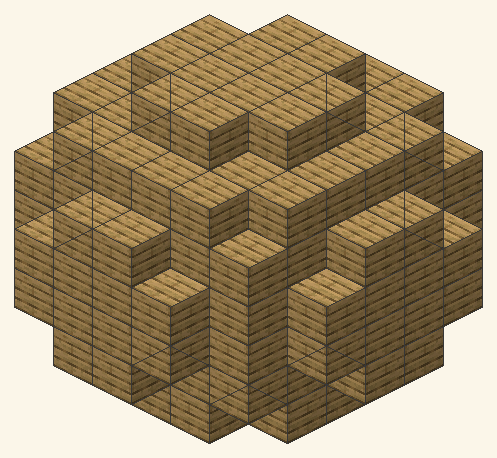
\includegraphics[width=\linewidth]{math_3d_tex_oak.png}
  \caption{\emph{Oak Planks}}
\end{subfigure}\hfill
\begin{subfigure}[t]{0.30\linewidth}\centering
  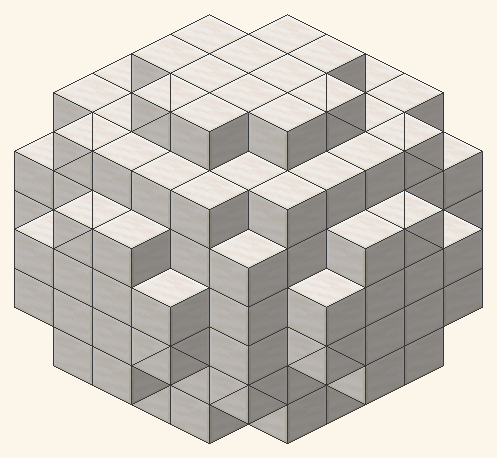
\includegraphics[width=\linewidth]{math_3d_tex_quartz.png}
  \caption{\emph{Quartz Block}}
\end{subfigure}
\caption{A mesma esfera de diâmetro $D=8$ renderizada com três blocos diferentes. A silhueta voxelizada (matemática) é idêntica nas três: o algoritmo escolhe os voxels, a textura é uma camada estética posterior que não altera nem o volume nem a topologia.}
\label{fig:textures}
\end{figure}

% =============================================================================
\section{Conclusão}

O presente documento descreveu, de forma sistemática, os fundamentos matemáticos empregados no Block Round. Em aproximadamente mil linhas de código JavaScript mais os pipelines de textura e áudio de suporte, o projeto integra contribuições de várias áreas teóricas:

\begin{itemize}[leftmargin=1.3em,itemsep=0.25em,topsep=0.4em]
  \item \acc{Geometria analítica}: equações implícitas da elipse e do elipsóide como critério primário de pertinência.
  \item \acc{Algoritmos clássicos de rasterização}: Bresenham na formulação de ponto médio, com extensão de Pitteway/Kappel para elipses.
  \item \acc{Topologia digital}: operadores de bordo discreto, conceitos de 4-, 6- e 26-conectividade, composição por fatias e contagem de faces expostas.
  \item \acc{Cálculo integral}: volume do elipsóide como integral tripla e sua contraparte discreta (medida de contagem sobre voxels).
  \item \acc{Álgebra linear}: planos de corte definidos por desigualdades lineares e projeção perspectiva tridimensional.
  \item \acc{Trigonometria}: parametrização da câmera em coordenadas esféricas e ajuste automático de distância em função do FOV.
  \item \acc{Aritmética combinatória de inventário}: contabilidade por divisão-com-teto de packs de $64$ e baús duplos de $3\,456$ itens, com a representação stacks-e-resto exibida pelo chip de info.
  \item \acc{Simetria de grupos}: exploração do grupo octaédrico $O_h$ e seu subgrupo de reflexões de ordem $8$ $\mathbb{Z}_2^3$ para reduzir o custo de construção por um fator de $8$ via \cmd{/clone}.
\end{itemize}

A observação central que o estudo permite formular é a seguinte: em uma malha discreta, \acc{não existe uma única representação correta} de uma curva contínua. Cada algoritmo apresentado neste documento corresponde a uma definição matemática distinta do critério de inclusão de células, e cada definição produz uma silhueta com propriedades formais próprias --- suavidade no algoritmo Euclidiano, padrão escalonado de Bresenham, maior abrangência no critério de cobertura por quina. A escolha do algoritmo, portanto, é uma decisão técnica que deve considerar o objetivo de representação visual pretendido, as características métricas desejadas para a forma resultante e --- especificamente para o Block Round --- o custo de inventário e de tempo de construir fisicamente a forma no jogo.

O Block Round ocupa um nicho pequeno mas matematicamente rico no ecossistema de ferramentas Minecraft: fica entre as ferramentas puramente geométricas (WorldEdit, Litematica) e as puramente visuais (resource packs, shaders), oferecendo uma ponte explícita, derivável e reproduzível da equação contínua até o plano de colocação discreto. O projeto irmão Pixel Round oferece os mesmos algoritmos sem a camada Minecraft, indicado para aplicações tradicionais de pixel art e voxel art. Juntos, os dois projetos exemplificam como o mesmo pipeline matemático contínuo-para-discreto sustenta workflows artísticos e construtivos radicalmente diferentes.

\clearpage

% =============================================================================
\section*{\color{accent}Apêndice A: Tabelas de referência de construção e exemplo prático}
\addcontentsline{toc}{section}{Apêndice A: Tabelas de referência de construção e exemplo prático}

Este apêndice reúne as referências numéricas e de comandos mais usadas pelos usuários do Block Round. Os dados abaixo consolidam as tabelas por seção e os exemplos práticos espalhados pelo documento, organizados para que o apêndice funcione como uma consulta de uma página para planejamento de construção, sintaxe de comandos e um exemplo prático completo.

\subsection*{A.1 Referência abrangente de esferas (preenchida, oca, packs)}
A tabela abaixo estende as tabelas canônicas de esfera das Seções~10 e~17 adicionando a variante de casca oca (modo \emph{fino}) ao lado do volume preenchido. As contagens de casca oca assumem uma casca de um único voxel e são computadas sob o algoritmo Euclidiano; o modo grosso adiciona cerca de $10{-}15\%$ mais blocos para preencher as células diagonais vazias conforme a Seção~12.

\vspace{0.4em}
\begin{center}
\begin{tabular}{@{}lrrrr@{}}
\toprule
\textbf{D} & \textbf{Preenchida (V)} & \textbf{Oca (casca)} & \textbf{Packs cheia} & \textbf{Packs oca} \\
\midrule
8   &   268 &   170 &  5  &  3  \\
10  &   523 &   316 &  9  &  5  \\
12  &   904 &   500 & 15  &  8  \\
14  &  1437 &   744 & 23  & 12  \\
16  &  2145 &  1042 & 34  & 17  \\
18  &  3052 &  1338 & 48  & 21  \\
20  &  4189 &  1648 & 66  & 26  \\
24  &  7238 &  2400 & 114 & 38  \\
28  & 11494 &  3296 & 180 & 52  \\
32  & 17156 &  4332 & 269 & 68  \\
\bottomrule
\end{tabular}
\end{center}

Para um construtor planejando uma run em survival, a coluna \emph{oca} costuma ser a relevante: apenas a casca visível precisa do bloco texturizado dedicado, enquanto o interior (se quiser algum) pode ser preenchido com o material mais barato. A coluna packs-cheia mostra o tamanho total de estoque para uma esfera totalmente preenchida; packs-oca é o mínimo realista para uma cúpula ou casca oca.

\subsection*{A.2 Referência de comandos WorldEdit / vanilla}
A tabela a seguir resume os comandos WorldEdit e do Minecraft vanilla mais relevantes para construir saídas do Block Round dentro do jogo. Comandos WorldEdit assumem que o jogador carrega uma varinha (machado de madeira por padrão) e selecionou uma região; comandos vanilla funcionam sem mod mas exigem argumentos de coordenadas.

\vspace{0.4em}
\begin{center}
\begin{tabular}{@{}lll@{}}
\toprule
\textbf{Comando} & \textbf{Mod / origem} & \textbf{Resultado} \\
\midrule
\cmd{//sphere stone 8}     & WorldEdit & esfera cheia r=8 (Euclidiana)  \\
\cmd{//hsphere stone 8}    & WorldEdit & esfera oca r=8 (só casca)  \\
\cmd{//cyl stone 8 16}     & WorldEdit & cilindro r=8, h=16  \\
\cmd{//ellipsoid st. 10 5 10} & WorldEdit & elipsóide 10\,$\times$\,5\,$\times$\,10  \\
\cmd{/fill ... stone}      & vanilla & preencher caixa com um tipo de bloco  \\
\cmd{/clone ... mode:masked} & vanilla & copiar região para novo local  \\
\bottomrule
\end{tabular}
\end{center}

Para usuários do Litematica o fluxo é diferente: em vez de rodar comandos, o arquivo schematic (Block Round exporta \code{.schem}, formato Sponge v2) é carregado no mod Litematica, que então exibe um fantasma translúcido da figura que o jogador coloca bloco a bloco. É o equivalente survival-mode mais próximo da experiência WorldEdit em creative.

\subsection*{A.3 Exemplo prático: cúpula D=20 de Quartzo sobre um templo}
Como exemplo prático completo, suponha que um construtor queira uma cúpula de Quartzo de $D=20$ no topo de um templo de pedra existente. O topo do templo é $11 \times 11$ blocos, centrado em $(0,80,0)$ nas coordenadas do mundo. A cúpula é a metade superior de uma esfera de raio $r=10$ cortada no plano $Y=0$. O plano de construção é:

\begin{enumerate}[leftmargin=1.6em,itemsep=0.3em,topsep=0.3em]
  \item \textbf{Planeje com Block Round.} Abra o app, defina modo 3D, Esfera, tamanho $D=20$, eixo de corte $Y$ a $50\%$. Selecione Bloco de Quartzo no picker. O chip de info reporta $V_{\mathrm{cupula}} \approx 2\,126$ blocos ($\approx 34$ packs, $1$ baú duplo com $1\,330$ itens sobrando no segundo).
  \item \textbf{Reúna recursos.} $34$ packs de Bloco de Quartzo = $\lceil 2\,126/4 \rceil = 532$ Blocos de Quartzo $\times 4$ Quartzo do Nether cada = $2\,128$ Quartzos do Nether. Funda ou comercie conforme apropriado.
  \item \textbf{Decida o algoritmo.} Para uma cúpula de Quartzo vista de baixo por transeuntes, o algoritmo Euclidiano dá a silhueta mais suave; para uma cúpula numa montanha remota, o algoritmo Limiar lê mais limpo. Block Round usa Euclidiano por padrão.
  \item \textbf{Posicione a cúpula.} A face plana da cúpula deve coincidir com o topo do templo. O bounding box da cúpula é $20 \times 10 \times 20$ blocos; coloque seu centro em $(0,80,0)$, de modo que a face plana (de corte) fique em $y=80$ e o ápice da cúpula fique em $y=89$.
  \item \textbf{Construa por simetria.} Construa o quadrante $+x, +z$ da cúpula (cerca de $\approx 530$ blocos). Emita \cmd{/clone 0 80 0 10 89 10 -10 80 0 mode:masked} para espelhar em $x$; depois \cmd{/clone -10 80 0 10 89 10 0 80 -10 mode:masked} para espelhar em $z$. Tempo decorrido total: $\sim 10$ minutos em survival.
  \item \textbf{Polimento.} Adicione Sea Lanterns no ápice e nos quatro pontos cardeais do equador para iluminação emissiva (Block Round renderiza esses blocos com seu emissive map no nível de luz MC $15$). Opcionalmente alterne o overlay de borda do Block Round (tecla \code{G}) para verificar que a casca da cúpula não tem buracos antes de colocar os últimos blocos.
\end{enumerate}

A matemática de cada passo é exatamente o que as vinte e duas seções anteriores descrevem: equação implícita do elipsóide, voxelização Euclidiana, corte no eixo Y, redução por simetria octaédrica via \cmd{/clone}, aritmética de inventário para traduzir o volume em packs e baús. O apêndice não é, portanto, uma teoria nova --- é um lembrete de que todo conceito teórico deste documento mapeia para uma decisão concreta e única no fluxo de planejamento de construção.

\subsection*{A.4 Referência de atalhos de teclado}

O app Block Round expõe um pequeno conjunto de atalhos de teclado que espelham os botões de canto no canvas. Estão listados abaixo para consulta rápida; os atalhos são globais (nenhum campo de input precisa estar em foco) e funcionam em modos 2D e 3D salvo nota em contrário.

\vspace{0.4em}
\begin{center}
\begin{tabular}{@{}lll@{}}
\toprule
\textbf{Tecla} & \textbf{Alterna} & \textbf{Notas} \\
\midrule
\code{G} & Overlay de borda  & contorno preto em cada face de voxel \\
\code{C} & Guias centrais  & cruz amarela translúcida nos eixos \\
\code{D} & Download PNG  & canvas atual como imagem PNG \\
\code{I} & Chip de info  & contagem de blocos e detalhe de packs \\
\code{M} & Alterna 2D / 3D  & troca entre modo plano e voxel \\
\code{S} & Som on/off  & sons ambientes de colocação \\
\code{T} & Tema dia / noite  & escurece fundo, mantém peças legíveis \\
\code{Ctrl+Z / Y} & Desfazer / refazer  & percorre o histórico de mudanças da figura \\
\bottomrule
\end{tabular}
\end{center}

Os atalhos \code{G} (grade) e \code{C} (guias centrais) são particularmente úteis durante a validação da construção: \code{G} mostra se cada voxel da casca está no lugar (um bloco faltante quebra o padrão do overlay), e \code{C} confirma que os cortes estão devidamente centrados nos eixos da figura.

Para o \code{Ctrl+Z} de desfazer: o Block Round percorre toda edição que muda a figura (sliders, modo de render, algoritmo, forma, eixo, bloco, alternância de modo) mas deliberadamente exclui alternâncias só visuais (câmera, edges overlay, cruz central, tema, som). Essa separação mantém a pilha de undo populada com edições que o usuário provavelmente vai querer reverter, não ajustes visuais casuais.

\subsection*{A.5 Glossário de termos-chave}

Referência rápida dos termos técnicos que se repetem por este documento. Cada entrada recapitula brevemente o conceito e aponta a seção onde é desenvolvido em detalhe.

\begin{itemize}[leftmargin=1.4em,itemsep=0.18em,topsep=0.3em]
  \item \textbf{Voxel} --- cubo unitário em 3D, análogo do pixel em 2D. Cada bloco de Minecraft é um voxel. Ver Seção~2.
  \item \textbf{Pack (stack)} --- em Minecraft, uma pilha de 64 itens idênticos ocupando um slot do inventário. Ver Seção~17.
  \item \textbf{Baú duplo} --- dois baús adjacentes fundidos em um container de 54 slots. Guarda até $3\,456$ itens. Ver Seção~17.
  \item \textbf{Shulker box} --- container portátil de 27 slots que pode ele mesmo ser guardado dentro de um slot de baú. Ver Seção~17.
  \item \textbf{Casca} --- a camada externa de um voxel de espessura de uma figura sólida. A superfície relevante para construtores de survival. Ver Seções~7 e~18.
  \item \textbf{Octante} --- uma das oito regiões do espaço 3D obtidas pela interseção dos três semiplanos coordenados. Usada na otimização por simetria. Ver Seção~20.
  \item \textbf{Mapeamento UV} --- uma parametrização 2D de uma face 3D, usada para mapear uma imagem de textura em cada face de um voxel. Ver Seção~21.
  \item \textbf{Bresenham} --- algoritmo incremental de rasterização de 1965 que usa apenas aritmética inteira. Ver Seção~5.
  \item \textbf{Limiar} --- critério de rasterização que inclui uma célula se alguma quina dela está dentro da elipse. Ver Seção~6.
  \item \textbf{Euclidiano} --- critério de rasterização que inclui uma célula se seu centro está dentro da elipse. Ver Seção~4.
  \item \textbf{Easter egg} --- recurso oculto disparado por uma entrada específica. No Block Round: a árvore de carvalho e o creeper, ambos no valor 15 do slider.
  \item \textbf{Schematic} --- arquivo de estrutura serializada (Sponge Schematic v2, \code{.schem}) carregável por WorldEdit, Litematica ou MCEdit.
\end{itemize}

Este glossário propositalmente fica mais curto do que um léxico matemático completo. Leitores que buscam cobertura mais profunda da matemática subjacente (topologia digital, cálculo integral, teoria de grupos, etc.) são remetidos às seções relevantes deste documento.

\subsection*{A.6 Perspectivas e limites do modelo}

O modelo do Block Round apresentado neste documento cobre a voxelização estática de elipses, elipsóides e seus cortes, além das considerações práticas introduzidas pela camada Minecraft. Não trata problemas dinâmicos --- figuras em movimento, transições de voxel animadas, interações com simulação de fluidos --- porque exigiriam um arcabouço de tempo contínuo fora do escopo da rasterização discreta. Uma extensão natural é a \emph{animação em nível de schematic}: uma sequência de voxelizações estáticas conectadas por interpolação, que o Block Round já consegue exportar como stream de \code{.schem} legível por scripts do Litematica.

Outra direção em aberto é a \emph{voxelização exata preservadora de volume}: a contagem discreta atual $V_{\mathrm{disc}}$ converge para o volume contínuo $V_{\mathrm{cont}}$ apenas assintoticamente. Para aplicações em que a contagem exata precise casar com a fórmula contínua (p.ex.\ competições de render, arte matemática com orçamentos rígidos de blocos), uma camada extra de refinamento é necessária --- por exemplo, ajustando levemente o raio para que a contagem discreta atinja o valor-alvo. O Block Round não implementa esse refinamento, mas a matemática é direta: resolver $V_{\mathrm{disc}}(r) = V_{\mathrm{alvo}}$ numericamente para $r$.

Por fim, a \emph{exploração de simetria de ordem superior}: este documento cobre o subgrupo de reflexões de ordem $8$ de $O_h$, mas o grupo completo de ordem $48$ inclui rotações que, em princípio, permitiriam um speedup de $\times 48$. O obstáculo prático é que os comandos no jogo operam em regiões alinhadas aos eixos, e explorar as simetrias rotacionais exige uma área de construção girada a $45°$. Mods do servidor que internamente rotacionam caixas de seleção (p.ex.\ FAWE) podem em princípio fazer isso, mas o tooling mainstream ainda não expõe. Uma implementação de referência demonstrando $\times 48$ num servidor vanilla seria um seguimento natural ao presente trabalho.

\subsection*{A.7 Referências adicionais e recursos externos}

Os conceitos matemáticos desenvolvidos neste documento têm literaturas bem estabelecidas. Para leitores que buscam fontes primárias ou maior profundidade algorítmica, recomendam-se os seguintes pontos de partida:

\begin{itemize}[leftmargin=1.4em,itemsep=0.2em,topsep=0.3em]
  \item J.~E.~Bresenham, \emph{Algorithm for computer control of a digital plotter}, IBM Systems Journal, vol.~4 no.~1, 1965 --- o artigo original de rasterização por aritmética inteira estendido neste documento.
  \item M.~L.~V.~Pitteway, \emph{Algorithm for drawing ellipses or hyperbolae with a digital plotter}, Computer Journal, vol.~10, 1967 --- generaliza Bresenham para cônicas arbitrárias.
  \item A.~Kappel, \emph{An ellipse-drawing algorithm for raster displays}, ACM Comm.\ vol.~28, 1985 --- a formulação elíptica de duas regiões usada na Seção~5.
  \item R.~Klette e A.~Rosenfeld, \emph{Digital Geometry: Geometric Methods for Digital Picture Analysis}, Morgan Kaufmann, 2004 --- referência padrão para topologia digital e os operadores de bordo das Seções~7 e~18.
  \item Documentação do WorldEdit, \emph{enginehub.org/worldedit/} --- referência oficial dos comandos \cmd{//sphere}, \cmd{//hsphere}, \cmd{//ellipsoid}, \cmd{//copy} usados ao longo deste documento.
  \item Especificação Sponge Schematic v2, \emph{github.com/SpongePowered/Schematic-Specification} --- o formato de arquivo que o Block Round exporta como \code{.schem}.
\end{itemize}

As oito áreas teóricas listadas na Seção~22 têm tratamentos em nível de livro-texto que vão muito além do que um único documento técnico pode resumir. A contribuição do Block Round não está na teoria em si mas na síntese específica: aplicar rasterização clássica ao cenário do Minecraft de voxels com textura, com as considerações explícitas de inventário e custo de simetria que normalmente são omitidas das ferramentas puramente geométricas.

Um comentário final sobre reprodutibilidade: todo o pipeline deste documento --- script de build, traduções, template LaTeX, tabelas por locale --- está contido no diretório \code{docs\_math/} do repositório do projeto. Re-executar \code{python build.py} num sistema com XeLaTeX/MiKTeX produz este PDF exatamente, em qualquer um dos nove locais suportados. O projeto irmão Pixel Round segue a mesma estrutura, permitindo comparação direta lado a lado das variantes texturizada e não-texturizada.

\vspace{1.2em}

\begin{center}
{\sffamily\bfseries\color{accent}Fim do documento}
\end{center}

\vspace{0.6em}

O Block Round é mantido por Vinícius Rodrigues de Souza. O projeto irmão Pixel Round está disponível em \emph{github.com/ViniSouza128/pixel-round}; o repositório atual do Block Round está em \emph{github.com/ViniSouza128/block-round}.

Comentários, correções e melhorias de tradução são bem-vindos pelo issue tracker do repositório do projeto. Revisão por falantes nativos das oito locales não-inglesas é particularmente valorizada, já que as localizações foram preparadas com revisão substancial mas a terminologia técnico-matemática se beneficia de correção nativa.

\end{document}
